% ==========================================================================
%  PFC 2026 (VF) - Versao Final
%  Planejamento de Trajetoria para Robo Terrestre Usando Grafos
%  Autores: Gabriel Dias Vilela e Tassandro Cavalcante Leitao
%  Instituto Militar de Engenharia
% ==========================================================================
\documentclass[
    12pt,
    openright,
    oneside,
    a4paper,
    english,
    brazil
]{abntex2}

% -- Pacotes --------------------------------------------------------------
\usepackage[utf8]{inputenc}
\usepackage[T1]{fontenc}
\usepackage{lmodern}
\usepackage{indentfirst}
\usepackage{graphicx}
\usepackage{microtype}
\usepackage{amsmath,amssymb}
\usepackage{booktabs}
\usepackage{multirow}
\usepackage{array}
\usepackage{hyperref}
\usepackage{float}
\usepackage{listings}
\usepackage{xcolor}
\usepackage{colortbl}
\usepackage{tikz}
\usetikzlibrary{positioning, arrows.meta, shapes.geometric, fit, backgrounds, calc}
\usepackage[brazilian,hyperpageref]{backref}
\usepackage[alf]{abntex2cite}

% -- Estilos TikZ globais para os diagramas do projeto ---------------------
\definecolor{boxBlue}{HTML}{2E86AB}
\definecolor{boxGreen}{HTML}{56B870}
\definecolor{boxOrange}{HTML}{E07B39}
\definecolor{boxPurple}{HTML}{8E5BB5}
\definecolor{boxGray}{HTML}{6C757D}
\definecolor{cinzaExec}{HTML}{A6A6A6}
\definecolor{cinzaPrev}{HTML}{E2E2E2}

\tikzset{
    pipelineBox/.style={
        rectangle, rounded corners=4pt, draw=#1, fill=#1!12, line width=0.9pt,
        minimum width=2.8cm, minimum height=1.5cm, align=center,
        inner sep=4pt, font=\small\sffamily, text=black
    },
    pipelineArrow/.style={
        -{Stealth[length=3mm, width=2mm]}, line width=0.9pt, draw=boxGray
    },
    compBox/.style={
        rectangle, rounded corners=3pt, draw=#1, fill=#1!10, line width=0.7pt,
        minimum width=5.6cm, minimum height=0.9cm, align=center,
        font=\footnotesize\sffamily, text=black
    },
    compTitle/.style={
        rectangle, rounded corners=3pt, fill=#1, line width=0.7pt,
        minimum width=5.6cm, minimum height=0.95cm, align=center,
        font=\small\bfseries\sffamily, text=white
    },
    compArrow/.style={
        -{Stealth[length=2.5mm, width=1.8mm]}, line width=0.7pt, draw=#1
    }
}

% -- Configuracao de listings ---------------------------------------------
\lstset{
    language=Python,
    basicstyle=\ttfamily\small,
    keywordstyle=\color{blue}\bfseries,
    stringstyle=\color{red},
    commentstyle=\color{gray}\itshape,
    numbers=left,
    numberstyle=\tiny\color{gray},
    breaklines=true,
    frame=single,
    captionpos=b,
}

% -- Dados do documento ---------------------------------------------------
\titulo{Planejamento de Trajetória para Robô Terrestre Usando Grafos}
\autor{Gabriel Dias Vilela \and Tassandro Cavalcante Leitão}
\local{Rio de Janeiro}
\data{2026}
\orientador{Claudia Marcela Justel, D.Sc.}
\coorientador{Paulo Fernando Ferreira Rosa, Ph.D.}
\instituicao{%
    MINISTÉRIO DA DEFESA\\
    EXÉRCITO BRASILEIRO\\
    DEPARTAMENTO DE CIÊNCIA E TECNOLOGIA\\
    INSTITUTO MILITAR DE ENGENHARIA\\
    CURSO DE GRADUAÇÃO EM ENGENHARIA DA COMPUTAÇÃO
}
\tipotrabalho{Projeto de Final de Curso}
\preambulo{Projeto de Final de Curso apresentado ao Curso de Graduação em Engenharia da Computação do Instituto Militar de Engenharia, como requisito parcial para a obtenção do título de Bacharel em Engenharia da Computação.}

% ==========================================================================
\begin{document}

\selectlanguage{brazil}
\frenchspacing

% ==========================================================================
%  ELEMENTOS PRE-TEXTUAIS
% ==========================================================================
\pretextual

% -- Capa -----------------------------------------------------------------
\begin{capa}
    \center
    \ABNTEXchapterfont

    {\normalsize
    MINISTÉRIO DA DEFESA\\
    EXÉRCITO BRASILEIRO\\
    DEPARTAMENTO DE CIÊNCIA E TECNOLOGIA\\
    INSTITUTO MILITAR DE ENGENHARIA\\
    CURSO DE GRADUAÇÃO EM ENGENHARIA DA COMPUTAÇÃO}

    \vspace*{2cm}

    {\large GABRIEL DIAS VILELA}\\
    {\large TASSANDRO CAVALCANTE LEITÃO}

    \vspace*{3cm}

    {\Large\bfseries PLANEJAMENTO DE TRAJETÓRIA PARA ROBÔ TERRESTRE USANDO GRAFOS}

    \vfill

    {\large RIO DE JANEIRO}\\
    {\large 2026}
\end{capa}

% -- Folha de rosto -------------------------------------------------------
\begin{folhaderosto}
    \center
    {\large GABRIEL DIAS VILELA}\\
    {\large TASSANDRO CAVALCANTE LEITÃO}

    \vspace*{3cm}

    {\Large\bfseries PLANEJAMENTO DE TRAJETÓRIA PARA ROBÔ TERRESTRE USANDO GRAFOS}

    \vspace*{2cm}

    \hspace{.45\textwidth}
    \begin{minipage}{.5\textwidth}
        \imprimirpreambulo\\[1em]
        Orientador(es): Claudia Marcela Justel, D.Sc.\\
        Paulo Fernando Ferreira Rosa, Ph.D.
    \end{minipage}

    \vfill

    {\large Rio de Janeiro}\\
    {\large 2026}
\end{folhaderosto}

% -- Ficha catalografica --------------------------------------------------
\begin{fichacatalografica}
    \vspace*{\fill}
    \begin{center}
    {\normalsize \copyright 2026\\
    INSTITUTO MILITAR DE ENGENHARIA\\
    Praça General Tibúrcio, 80 -- Praia Vermelha\\
    Rio de Janeiro -- RJ CEP: 22290-270}
    \end{center}

    \vspace{1cm}

    \noindent Este exemplar é de propriedade do Instituto Militar de Engenharia, que poderá incluí-lo em base de dados, armazenar em computador, microfilmar ou adotar qualquer forma de arquivamento.

    É permitida a menção, reprodução parcial ou integral e a transmissão entre bibliotecas deste trabalho, sem modificação de seu texto, em qualquer meio que esteja ou venha a ser fixado, para pesquisa acadêmica, comentários e citações, desde que sem finalidade comercial e que seja feita a referência bibliográfica completa.

    Os conceitos expressos neste trabalho são de responsabilidade do(s) autor(es) e do(s) orientador(es).

    \vspace{1cm}

    \noindent
    Dias Vilela, Gabriel; Cavalcante Leitão, Tassandro.\\
    Planejamento de trajetória para robô terrestre usando grafos / Gabriel Dias Vilela e Tassandro Cavalcante Leitão. -- Rio de Janeiro, 2026.\\
    XX f.\\[0.5em]
    Orientador(es): Claudia Marcela Justel e Paulo Fernando Ferreira Rosa.\\[0.5em]
    Projeto de Final de Curso (graduação) -- Instituto Militar de Engenharia, Engenharia da Computação, 2026.\\[0.5em]
    1.~Veículos terrestres não tripulados. 2.~Segmentação semântica. 3.~Algoritmos baseados em grafos. 4.~Planejamento de trajetórias. 5.~Robot Operating System. i.~Justel, Claudia Marcela (orient.) ii.~Ferreira Rosa, Paulo Fernando (orient.) iii.~Título
    \vspace*{\fill}
\end{fichacatalografica}

% -- Folha de aprovacao ---------------------------------------------------
\begin{folhadeaprovacao}
    \center

    {\large GABRIEL DIAS VILELA}\\
    {\large TASSANDRO CAVALCANTE LEITÃO}

    \vspace{1cm}

    {\large\bfseries Planejamento de trajetória para robô terrestre usando grafos}

    \vspace{1cm}

    Projeto de Final de Curso apresentado ao Curso de Graduação em Engenharia da Computação do Instituto Militar de Engenharia, como requisito parcial para a obtenção do título de Bacharel em Engenharia da Computação.

    \vspace{0.5cm}

    Orientador(es): Claudia Marcela Justel e Paulo Fernando Ferreira Rosa.

    \vspace{0.5cm}

    Aprovada em \_\_\_ de \_\_\_\_\_\_\_\_\_\_\_ de 2026, pela seguinte banca examinadora:

    \vspace{1.5cm}

    \assinatura{Prof. Paulo Fernando Ferreira Rosa -- Professor do IME -- Presidente}
    \assinatura{Profa. Claudia Marcela Justel -- Professora do IME}
    \assinatura{Membro 3 -- Instituição}
    \assinatura{Membro 4 -- Instituição}
    \assinatura{Membro 5 -- Instituição}

    \vfill

    {\large Rio de Janeiro}\\
    {\large 2026}
\end{folhadeaprovacao}

% -- Dedicatoria ----------------------------------------------------------
\begin{dedicatoria}
    \vspace*{\fill}
    \centering
    \noindent
    \textit{Às nossas famílias.}
    \vspace*{\fill}
\end{dedicatoria}

% -- Agradecimentos -------------------------------------------------------
\begin{agradecimentos}
Os agradecimentos principais são direcionados aos nossos orientadores por todo acompanhamento e ensinamentos. Agradecemos também ao Major Fábio Luiz Junior, cujos modelos de segmentação e trabalho de referência sobre planejamento em mapas de navegabilidade fundamentam este projeto, e aos autores do projeto anterior, João Vitor Camelo de Almeida e Thiago Calheiros de Souza Barbosa, cujo trabalho serviu de base e inspiração para o presente projeto.
\end{agradecimentos}

% -- Epigrafe -------------------------------------------------------------
\begin{epigrafe}
    \vspace*{\fill}
    \begin{flushright}
        \textit{``Não vos amoldeis às estruturas deste mundo,\\
        mas transformai-vos pela renovação da mente,\\
        a fim de distinguir qual é a vontade de Deus:\\
        o que é bom, o que Lhe é agradável, o que é perfeito.''}\\
        (Bíblia Sagrada, Romanos 12, 2)
    \end{flushright}
\end{epigrafe}

% -- Resumo ---------------------------------------------------------------
\setlength{\absparsep}{18pt}
\begin{resumo}
Este trabalho é a versão final do Projeto de Final de Curso de planejamento de trajetória para veículos terrestres não tripulados (UGV), conduzido em continuidade ao projeto de mesmo tema desenvolvido em 2025 por outra dupla de alunos. O projeto foi entregue em três etapas. A primeira entrega definiu o escopo, projetou uma arquitetura de \textit{software} modular e orientada a objetos, organizada em cinco estágios encadeados (ingestão de dados, pré-processamento, construção de grafos, algoritmos e pós-processamento), e implementou os algoritmos de busca em grafos BFS, DFS, Dijkstra e A* sobre o cálculo de rotas diretamente na imagem. A segunda entrega consolidou três acréscimos: a inclusão do algoritmo \textit{Rapidly-exploring Random Tree} (RRT) ao catálogo de planejadores, a integração de modelos de segmentação semântica pré-treinados (U-Net) sobre o \textit{Semantic Drone Dataset} \cite{drone_dataset} e disponibilizados em \cite{junior2024_models}, e a ligação do pós-processamento ao \textit{Robot Operating System} (ROS 2) \cite{quigley2009} para simulação do movimento no Gazebo \cite{koenig2004}. Esta versão final consolida os resultados experimentais das três frentes, acrescenta a geração automática de mapas de ocupação a partir da descrição do mundo simulado, de modo que o caminho planejado e o mundo do simulador compartilhem o mesmo referencial métrico, e apresenta a caracterização quantitativa dos percursos executados pelo UGV simulado (Clearpath Jackal). Os ensaios em ambiente virtual foram concluídos com êxito: o robô simulado percorre integralmente as trajetórias planejadas, tanto sobre mapas de ocupação do próprio simulador quanto sobre imagens aéreas reais obtidas por UAV. A validação em ambiente real, prevista no cronograma, não pôde ser realizada dentro do prazo do projeto por restrições de acesso a plataforma física, de espaço de ensaio e de tempo, e permanece como a etapa imediata de continuidade.

\textbf{Palavras-chave}: Veículos terrestres não tripulados; Segmentação semântica; Algoritmos baseados em grafos; Planejamento de trajetórias; RRT; ROS; Simulador Gazebo.
\end{resumo}

% -- Abstract -------------------------------------------------------------
\begin{resumo}[Abstract]
\begin{otherlanguage*}{english}
This work is the final version of the undergraduate final project on trajectory planning for unmanned ground vehicles (UGV), carried out as a continuation of the project on the same subject developed in 2025 by a different pair of students. The project was delivered in three stages. The first delivery defined the scope, designed a modular object-oriented software architecture organized into five chained stages (data ingestion, preprocessing, graph construction, algorithms, and post-processing), and implemented the BFS, DFS, Dijkstra, and A* graph-search algorithms over image-based route computation. The second delivery consolidated three additions: the inclusion of the Rapidly-exploring Random Tree (RRT) algorithm in the planner catalog, the integration of semantic segmentation models (U-Net) pre-trained on the Semantic Drone Dataset \cite{drone_dataset} and released in \cite{junior2024_models}, and the connection of the post-processing stage to the Robot Operating System (ROS 2) \cite{quigley2009} for motion simulation in Gazebo \cite{koenig2004}. This final version consolidates the experimental results of the three fronts, adds the automatic generation of occupancy maps from the description of the simulated world, so that the planned path and the simulator world share the same metric frame, and presents the quantitative characterization of the routes executed by the simulated UGV (Clearpath Jackal). The virtual environment trials were completed successfully: the simulated robot drives the full planned trajectories, both over occupancy maps of the simulator itself and over real aerial imagery acquired by a UAV. Validation in a real environment, foreseen in the schedule, could not be carried out within the project deadline due to restrictions on access to a physical platform, on test area, and on time, and remains the immediate continuation step.

\textbf{Keywords}: Unmanned ground vehicles; Semantic segmentation; Graph-based algorithms; Trajectory planning; RRT; ROS; Gazebo simulator.
\end{otherlanguage*}
\end{resumo}

% -- Listas ---------------------------------------------------------------
\pdfbookmark[0]{\listfigurename}{lof}
\listoffigures*
\cleardoublepage

\pdfbookmark[0]{\listtablename}{lot}
\listoftables*
\cleardoublepage

% -- Lista de abreviaturas e siglas ---------------------------------------
\begin{siglas}
    \item[BFS] Breadth-First Search
    \item[CNN] Convolutional Neural Network
    \item[CTEx] Centro Tecnológico do Exército
    \item[DDS] Data Distribution Service
    \item[DFS] Depth-First Search
    \item[EB] Exército Brasileiro
    \item[EKF] Extended Kalman Filter
    \item[GSD] Ground Sampling Distance
    \item[IA] Inteligência Artificial
    \item[mIoU] Mean Intersection over Union
    \item[OOP] Object-Oriented Programming
    \item[PFC] Projeto de Final de Curso
    \item[QoS] Quality of Service
    \item[ROS] Robot Operating System
    \item[RRT] Rapidly-exploring Random Tree
    \item[SDD] Semantic Drone Dataset
    \item[SDF] Simulation Description Format
    \item[SVTRP] Sistemas de Veículos Terrestres Remotamente Pilotados
    \item[UAV] Unmanned Aerial Vehicle
    \item[UGV] Unmanned Ground Vehicle
    \item[VC] Segunda entrega deste Projeto de Final de Curso
    \item[VE] Primeira entrega deste Projeto de Final de Curso
    \item[VF] Entrega final deste Projeto de Final de Curso
    \item[WSL] Windows Subsystem for Linux
\end{siglas}

% -- Sumario --------------------------------------------------------------
\pdfbookmark[0]{\contentsname}{toc}
\tableofcontents*
\cleardoublepage

% ==========================================================================
%  ELEMENTOS TEXTUAIS
% ==========================================================================
\textual

% ======================================================================
\chapter{INTRODUÇÃO}
% ======================================================================

Os avanços tecnológicos envolvendo visão computacional, eletrônica e inteligência artificial, entre outras áreas correlatas, impulsionaram a tendência de desenvolvimento e uso de ferramentas que automatizam as disputas em ambientes de combate. Nesse sentido, com a possibilidade de aumentar a eficácia operacional e reduzir a participação e desgaste humano (física, cognitiva e psicologicamente) no campo de batalha, a integração de robôs autônomos nesses cenários de confronto é iminente e torna-se motivo de vantagem tática e estratégica.

Em relação à autonomia desses sistemas, o planejamento de trajetória de robôs terrestres é uma das tarefas essenciais a ser realizada e ela se encontra dentro de um escopo multidisciplinar que inclui conhecimentos em diversas áreas de grande complexidade, como a robótica e a teoria dos grafos. Essas disciplinas convergem na modelagem do cenário de combate como um grafo, no qual os nós representam as posições transitáveis pelos robôs no mapa e as arestas definem os caminhos. Dessa maneira, algoritmos de busca e otimização são ferramentas que guiam o planejamento das possíveis rotas, auxiliando na coordenação entre pontos e adaptação aos obstáculos.

A pesquisa ``Cooperação Entre Plataformas Terrestres e Aéreas para Aquisição, Rastreamento e Perseguição de Alvos, Utilizando Visão Computacional e Inteligência Artificial'' \cite{junior2024}, que se encontra em fase de desenvolvimento no laboratório LIARC, iniciada em 2023 pelo Major Fábio Luiz Junior, aborda o emprego de plataformas robóticas aéreas (UAV) e terrestres (UGV) em ambientes de batalha e como essas duas estruturas podem trabalhar em conjunto para otimizar e ampliar o poder de ataque e estratégico militar.

% -- 1.1 -------------------------------------------------------------------
\section{Convenções de Nomenclatura Adotadas neste Texto}
\label{sec:nomenclatura}

Este projeto tem duas origens distintas que precisam ser diferenciadas ao longo do texto: um trabalho anterior, conduzido por outros alunos, e as entregas parciais deste próprio projeto. Para evitar ambiguidade, adotam-se as seguintes convenções, usadas de forma uniforme em todos os capítulos:

\begin{itemize}
    \item \textbf{PFC 2025}, ou ``o projeto do ano anterior'': refere-se exclusivamente ao trabalho ``Planejamento de Trajetória para Robô Terrestre, Utilizando Otimização em Grafos'', defendido em 2025 por João Vitor Camelo de Almeida e Thiago Calheiros de Souza Barbosa \cite{camelo2025}. Trata-se de outro Projeto de Final de Curso, de outra dupla, do qual o presente trabalho é continuação;
    \item \textbf{VE}, ou ``primeira versão deste projeto'': primeira das três entregas deste Projeto de Final de Curso, de caráter de planejamento e estruturação, descrita na Seção~\ref{sec:evolucao};
    \item \textbf{VC}, ou ``segunda versão deste projeto'': segunda entrega deste Projeto de Final de Curso, na qual as propostas da VE foram implementadas e integradas;
    \item \textbf{VF}, ou ``esta versão final'': a presente entrega, que consolida os resultados e encerra o projeto.
\end{itemize}

Sempre que o texto mencionar ``o projeto anterior'' sem qualificação adicional, a referência é ao PFC 2025 \cite{camelo2025}. Quando a referência for a uma entrega anterior deste mesmo projeto, o texto usará explicitamente ``VE'', ``primeira versão'', ``VC'' ou ``segunda versão''.

% -- 1.2 -------------------------------------------------------------------
\section{Contribuições do PFC 2025}
\label{sec:pfc2025}

O presente projeto é uma continuação direta do PFC 2025 \cite{camelo2025}. Naquele trabalho, os autores propuseram uma abordagem baseada em grafos para o planejamento de caminhos sobre imagens aéreas já segmentadas, implementando os algoritmos de Dijkstra e A* e comparando-os com o algoritmo estocástico RRT.

As principais conclusões do PFC 2025 foram:

\begin{itemize}
    \item Os algoritmos baseados em grafos (Dijkstra e A*) apresentaram desempenho mais consistente, confiável e previsível em relação ao RRT, destacando-se pelo determinismo e pela garantia de otimalidade das soluções;
    \item O algoritmo A* mostrou-se ligeiramente mais rápido que o Dijkstra, explorando um menor número de nós, sendo considerado mais adequado ao problema proposto;
    \item A inserção de pesos nas arestas do grafo, com base na proximidade a obstáculos, produziu caminhos mais realistas que se distanciam de regiões de risco, sem impacto significativo no tempo de execução;
    \item O RRT apresentou dificuldades em imagens com áreas transitáveis estreitas, excedendo o tempo limite em dois dos cinco cenários testados;
    \item A abordagem proposta, ao integrar segmentação semântica de imagens e planejamento baseado em grafos, constitui uma alternativa promissora para aplicações em veículos autônomos.
\end{itemize}

O PFC 2025 apontou três frentes de continuidade: o tratamento de ambientes dinâmicos, a avaliação do uso de grafos em composição de imagens em tempo real e a extensão da segmentação semântica para uma variedade maior de terrenos. Este projeto concentrou-se na terceira frente e acrescentou uma quarta, não prevista naquele trabalho: a execução efetiva do caminho planejado por um veículo, ainda que simulado.

% -- 1.3 -------------------------------------------------------------------
\section{Da Primeira Versão à Versão Final deste Projeto}
\label{sec:evolucao}

Este Projeto de Final de Curso foi conduzido em três entregas, conforme a nomenclatura da Seção~\ref{sec:nomenclatura}.

A \textbf{primeira versão (VE)} teve caráter de planejamento e de estruturação. Ela definiu o escopo do trabalho, projetou a arquitetura de \textit{software} modular e orientada a objetos (cinco módulos encadeados, com interfaces abstratas e padrões de fábrica) e implementou os algoritmos-base de busca em grafos (BFS, DFS, Dijkstra e A*) sobre um sistema de cálculo de rotas diretamente na imagem, tomando como entrada um mapa de navegabilidade com cores fixas. Naquele estágio, a segmentação semântica e a validação em simulação foram apresentadas como propostas de arquitetura, ainda não implementadas.

A \textbf{segunda versão (VC)} transformou aquelas propostas em componentes efetivamente implementados e integrados ao \textit{pipeline}, além de ampliar o catálogo de planejadores. Os três acréscimos centrais foram:

\begin{enumerate}
    \item \textbf{Inclusão do algoritmo RRT.} O planejador baseado em amostragem \textit{Rapidly-exploring Random Tree} \cite{lavalle1998} foi adicionado ao catálogo de algoritmos, ao lado de BFS, DFS, Dijkstra e A*, sob a mesma interface. Isso permite contrastar diretamente, sobre os mesmos mapas, o comportamento de um planejador estocástico com o dos algoritmos determinísticos de busca em grafos, retomando de forma integrada a comparação iniciada no PFC 2025 \cite{camelo2025}.

    \item \textbf{Implementação da segmentação semântica.} A identificação das áreas transitáveis, antes dependente de mapas previamente segmentados, passou a ser realizada dentro do próprio \textit{pipeline} por meio dos modelos U-Net pré-treinados disponibilizados em \cite{junior2024_models}, treinados sobre o \emph{Semantic Drone Dataset} \cite{drone_dataset}. O módulo de pré-processamento executa a rede sobre a imagem RGB do UAV e produz um mapa de navegabilidade pronto para a conversão em grafo.

    \item \textbf{Integração com ROS 2 e simulação do movimento no Gazebo.} O módulo de pós-processamento foi estendido com uma ponte para o ROS 2 \cite{quigley2009}, que publica a imagem anotada e a trajetória calculada; do lado do robô, um conjunto de nós ROS 2 faz um UGV simulado (Clearpath Jackal) percorrer efetivamente essa trajetória no Gazebo \cite{koenig2004}.
\end{enumerate}

Esta \textbf{versão final (VF)} tem três objetivos próprios, que a distinguem da VC:

\begin{enumerate}
    \item \textbf{Consolidar a avaliação dos percursos simulados.} Na VC, a integração com o Gazebo havia sido verificada apenas qualitativamente, isto é, constatou-se que o robô percorria o caminho até o destino. Esta versão registra os percursos executados, com extensão, duração e velocidade média, discute a aderência observada entre a trajetória planejada e a percorrida e trata o efeito do fator de escala em metros por pixel, conforme a Seção~\ref{sec:res_gazebo}.

    \item \textbf{Alinhar o referencial do planejamento ao do mundo simulado.} Foi acrescentada uma ferramenta que converte a descrição do mundo do Gazebo, no formato SDF, em um mapa de ocupação bidimensional no mesmo padrão de cores consumido pelo \textit{pipeline}. Com isso, o caminho é planejado sobre a geometria real do mundo em que o robô vai andar, e não sobre uma imagem sem relação métrica com ele. Esse acréscimo é descrito na Seção~\ref{sec:mapa_ocupacao}.

    \item \textbf{Registrar o estágio final do projeto, inclusive o que não foi concluído.} O cronograma previa, para o encerramento, uma validação em ambiente real, com um veículo físico. Essa etapa não foi realizada. As razões, de ordem material e de prazo, e a discussão de como retomá-la estão na Seção~\ref{sec:limitacoes} e no Capítulo~\ref{cap:conclusao}.
\end{enumerate}

% -- 1.4 -------------------------------------------------------------------
\section{Motivação e Justificativa}

O presente projeto busca dar continuidade e aprofundar o estudo de planejamento de rotas abordado em \cite{camelo2025} e \cite{junior2024} e que, por sua vez, poderá ser aproveitado e aplicado no projeto estratégico ``Sistemas de Veículos Terrestres Remotamente Pilotados'' (SVTRP), conduzido pelo Centro Tecnológico do Exército (CTEx), visando a uma potencialização de seu funcionamento.

O PFC 2025 demonstrou a viabilidade da abordagem baseada em grafos, porém dependia de imagens previamente segmentadas e não contemplava a execução dos caminhos em um robô. A necessidade de integrar o processo de segmentação diretamente no \textit{pipeline}, utilizando modelos especializados em imagens de drones, e de validar os caminhos em um veículo simulado constitui a principal motivação das duas últimas entregas. A adoção dos modelos pré-treinados disponibilizados em \cite{junior2024_models} permite reutilizar diretamente o conhecimento já validado em pesquisa anterior do laboratório \cite{junior2024}, evitando o retreinamento e mantendo coerência com a linha de trabalho do CTEx.

Adicionalmente, a inclusão do RRT ao catálogo dá base experimental para discutir, sobre os mesmos cenários, os compromissos entre planejadores determinísticos e estocásticos. Por fim, a integração com o Gazebo, motivada pelo objetivo de validar os caminhos antes de qualquer implantação em campo, fecha o ciclo entre o planejamento e a execução do movimento em um UGV. Um caminho ótimo sobre uma imagem não é, por si só, garantia de que um veículo com dinâmica própria consiga percorrê-lo, e a simulação é a forma de verificar isso sem risco e sem custo de plataforma.

% -- 1.5 -------------------------------------------------------------------
\section{Objetivos}

O objetivo principal deste Projeto de Final de Curso consiste em construir um sistema modular capaz de, a partir de uma imagem aérea real, identificar as áreas transitáveis, planejar uma trajetória por diferentes algoritmos e executar essa trajetória em um veículo terrestre, validando-a previamente em ambiente simulado.

Para atingir o objetivo principal, foram definidos os seguintes objetivos específicos:

\begin{itemize}
    \item Projetar e implementar uma arquitetura orientada a objetos composta por cinco módulos encadeados: ingestão de dados, pré-processamento, construção de grafos, algoritmos e pós-processamento (concluído na VE);
    \item Incorporar o algoritmo RRT ao módulo de algoritmos, sob a mesma interface dos demais planejadores, e compará-lo com BFS, DFS, Dijkstra e A* sobre os mesmos mapas (concluído na VC);
    \item Implementar o módulo de segmentação semântica com os modelos pré-treinados de \cite{junior2024_models}, gerando mapas de navegabilidade no formato adotado em \cite{junior2025_rrt} a partir de imagens RGB reais de drone (concluído na VC);
    \item Estender o pós-processamento com uma ponte ROS 2 e integrar um UGV simulado (Clearpath Jackal) no Gazebo (concluído na VC);
    \item Caracterizar, em simulação, os percursos executados pelo veículo e tratar a correspondência métrica entre a imagem de planejamento e o mundo simulado (concluído nesta VF);
    \item Validar o sistema em ambiente real, com um veículo físico (não realizado, conforme a Seção~\ref{sec:limitacoes}).
\end{itemize}

% -- 1.6 -------------------------------------------------------------------
\section{Metodologia}

Visando alcançar os objetivos propostos, a metodologia adotada consistiu nas seguintes etapas. Inicialmente, foi conduzida uma revisão do PFC 2025 \cite{camelo2025} e da literatura relacionada a segmentação semântica de imagens aéreas, planejamento de trajetórias e simulação robótica. Em seguida, sobre a arquitetura modular definida na primeira versão, foram implementados os três acréscimos da segunda versão: o algoritmo RRT foi adicionado ao módulo \texttt{algorithm}; o módulo \texttt{preprocessing} passou a executar os modelos de segmentação de \cite{junior2024_models}; e o módulo \texttt{post\_processing} foi acoplado a uma ponte ROS 2 que alimenta a simulação no Gazebo.

Nesta versão final, os testes foram organizados em três frentes. A primeira compara os modelos de segmentação sobre as mesmas imagens aéreas, medindo a fração de área classificada como transitável e o tempo de inferência. A segunda compara os cinco planejadores sobre um mesmo grafo, com os mesmos pontos de origem e destino, registrando número de nós do caminho, custo, nós explorados, tempo e comprimento geométrico. A terceira executa a trajetória planejada em um UGV simulado, tanto sobre mapas de ocupação extraídos do próprio mundo do simulador quanto sobre imagens aéreas reais, e compara o percurso realizado com o planejado.

% -- 1.7 -------------------------------------------------------------------
\section{Estrutura}

Este documento está organizado da seguinte forma. No Capítulo~2, são apresentados os conceitos preliminares que fundamentam o projeto, incluindo grafos, algoritmos de caminhos mínimos, o planejamento por amostragem (RRT), a segmentação semântica e a simulação robótica com ROS e Gazebo. No Capítulo~3, descreve-se a arquitetura do sistema e o detalhamento das implementações. O Capítulo~4 é dedicado à apresentação e discussão dos resultados experimentais, incluindo as limitações encontradas. No Capítulo~5, são apresentadas as conclusões e as perspectivas futuras. O Capítulo~6 apresenta o cronograma das atividades e o seu grau de cumprimento. Por fim, antes das referências, é apresentada a declaração sobre o uso de ferramentas de inteligência artificial na elaboração deste trabalho.

% ======================================================================
\chapter{CONCEITOS PRELIMINARES}
% ======================================================================

Neste capítulo, apresentamos os conceitos fundamentais necessários para a compreensão do projeto. Além dos tópicos já abordados no PFC 2025 \cite{camelo2025}, que são veículos terrestres autônomos, planejamento de caminhos, grafos e algoritmos clássicos, introduzimos os conceitos relacionados ao que foi acrescentado ao longo deste projeto: o planejamento por amostragem (RRT), a segmentação semântica e a simulação robótica com ROS e Gazebo.

% -- 2.1 -------------------------------------------------------------------
\section{Veículos Terrestres Autônomos}

Segundo \cite{finn2010}, um veículo terrestre autônomo (UGV) é um sistema robótico complexo e multidisciplinar, com participação ostensiva das engenharias mecânica, da computação e eletrônica. Este sistema tem como objetivo navegar pelo terreno de forma autônoma, sem a necessidade de intervenção por um operador externo, e executar determinada tarefa. Nos últimos anos, evidencia-se grande crescimento nas aplicações de UGVs, desde aplicações civis até aplicações militares.

O veículo adotado como plataforma de demonstração neste trabalho, o Clearpath Jackal, é um UGV de pequeno porte com tração diferencial. Nesse tipo de tração, as rodas de cada lado do veículo são acionadas de forma independente, de modo que o robô controla apenas duas grandezas: a velocidade linear $v$, ao longo do próprio eixo longitudinal, e a velocidade angular $\omega$, em torno do eixo vertical. O veículo não consegue transladar lateralmente. Essa restrição é relevante para o planejamento, porque um caminho geometricamente curto mas com mudanças bruscas de direção obriga o veículo a parar, girar e retomar o movimento, o que aumenta o tempo de percurso mesmo sem aumentar a distância.

% -- 2.2 -------------------------------------------------------------------
\section{Planejamento de Caminhos}

O planejamento de caminhos é considerado um desafio crítico em Inteligência Artificial e essencial para o movimento autônomo de todos os sistemas inteligentes, como veículos terrestres \cite{madridano2021}. O planejamento pode ser categorizado como global (estático), quando toda a informação sobre o ambiente é conhecida, ou local (dinâmico), quando o ambiente é parcialmente desconhecido \cite{chen2020}. Neste trabalho, abordamos o planejamento de caminhos globais: supõe-se que a imagem aérea, capturada previamente por um UAV, descreve por completo o ambiente em que o UGV vai operar.

% -- 2.3 -------------------------------------------------------------------
\section{Grafos}

Um grafo $G = (V, E)$ consiste em um conjunto finito de vértices $V = \{v_1, v_2, \ldots, v_n\}$ e um conjunto finito de arestas $E = \{e_1, e_2, \ldots, e_m\}$, com $m, n \in \mathbb{N}$, tal que cada aresta é identificada com um par de vértices $(v_i, v_j)$ \cite{chen1997}. Podemos classificar os grafos como ponderados, caso suas arestas possuam pesos associados, ou não ponderados, caso contrário.

Neste projeto, o grafo não é fornecido: ele é construído a partir de uma imagem. Cada pixel classificado como transitável vira um vértice, e dois vértices são ligados por uma aresta quando os pixels correspondentes são vizinhos na imagem. A noção de vizinhança usada é um parâmetro do sistema, chamado de \emph{conectividade}:

\begin{itemize}
    \item \textbf{Conectividade 4}: cada pixel é ligado apenas aos vizinhos acima, abaixo, à esquerda e à direita. Os caminhos resultantes só têm segmentos horizontais e verticais, o que produz trajetórias em forma de escada;
    \item \textbf{Conectividade 8}: acrescentam-se as quatro diagonais. Os caminhos ficam mais próximos de retas, ao custo de aproximadamente o dobro de arestas.
\end{itemize}

Neste trabalho utiliza-se conectividade 8, por produzir caminhos mais próximos do que um veículo real percorreria. A ordem de grandeza dos grafos envolvidos é relevante: uma imagem de $1000 \times 750$ pixels com a maior parte da área transitável gera algumas centenas de milhares de vértices e alguns milhões de arestas. É por isso que a eficiência da construção do grafo, discutida na Seção~\ref{sec:construcao_grafos}, importa tanto quanto a eficiência do algoritmo de busca.

A representação enriquecida de grafo adotada neste projeto, com atributos associados a nós e arestas, é detalhada na Seção~\ref{sec:construcao_grafos}, junto à construção do grafo.

% -- 2.4 -------------------------------------------------------------------
\section{Algoritmos de Caminhos Mínimos em Grafos}
\label{sec:caminhos_minimos}

A definição de caminho mínimo entre dois vértices apoia-se em duas noções básicas da teoria dos grafos \cite{deo2016, chen1997}. Um \emph{caminho} de um vértice $u$ para um vértice $v$ em um grafo $G = (V, E)$ é uma sequência alternada de vértices e arestas
\[
P = (v_0, e_1, v_1, e_2, v_2, \ldots, e_k, v_k),
\]
com $v_0 = u$, $v_k = v$, $e_i = (v_{i-1}, v_i) \in E$ para todo $i$ e sem repetição de vértices. O \emph{comprimento} do caminho $P$ em um grafo ponderado é a soma dos pesos das suas arestas:
\[
\ell(P) = \sum_{i=1}^{k} w(e_i),
\]
onde $w : E \to \mathbb{R}_{\geq 0}$ é a função de pesos do grafo. No caso não ponderado, define-se $w(e_i) = 1$ para toda aresta, de modo que o comprimento coincide com o número de arestas do caminho.

O \emph{problema do caminho mínimo} entre $u$ e $v$ consiste, então, em determinar um caminho $P^\ast$ tal que
\[
\ell(P^\ast) = \min \{\, \ell(P) : P \text{ é caminho de } u \text{ a } v \,\}.
\]

Duas observações são importantes para a leitura dos resultados do Capítulo~\ref{cap:resultados}. A primeira é que o caminho mínimo não é necessariamente único: em um grafo em grade, é comum existirem muitos caminhos distintos com exatamente o mesmo custo. Dois algoritmos corretos podem, portanto, devolver caminhos diferentes e ambos estarem certos. A segunda é que ``comprimento'' no sentido da função $\ell$ acima é o custo acumulado, que neste projeto embute uma penalização por proximidade a obstáculos, e não a distância geométrica em pixels. As duas grandezas são reportadas separadamente nas tabelas de resultados.

No contexto deste projeto, o grafo é construído a partir do mapa de navegabilidade gerado pela segmentação semântica, e o caminho mínimo corresponde à trajetória de menor custo entre o ponto inicial e o ponto final escolhidos pelo operador.

A seguir, são apresentados os quatro algoritmos clássicos de busca em grafos implementados neste projeto. Em todos eles, chama-se \emph{nó explorado} (ou expandido) aquele que foi retirado da estrutura de busca e teve os seus vizinhos examinados. Esse número é uma medida do trabalho realizado pelo algoritmo que não depende da máquina em que ele é executado, ao contrário do tempo de execução medido em segundos.

\subsection{Breadth-First Search (BFS)}

A BFS é um algoritmo que permite percorrer vértices e arestas em grafos \cite{cormen2009, moore1959}. Iniciando o percurso em um nó denominado fonte, a busca se expande visitando os nós em uma mesma profundidade antes de avançar. Sua particularidade, buscar em largura, permite determinar caminhos mínimos em grafos não ponderados de maneira eficiente, com complexidade $O(|V| + |E|)$.

No contexto deste projeto, a BFS minimiza o número de arestas do caminho, e não o custo. Como cada aresta corresponde a um passo de um pixel, o caminho da BFS é o que usa menos passos e, por isso, tende a ser o geometricamente mais curto. Em compensação, ele ignora por completo a penalização por proximidade a obstáculos, e por isso costuma passar rente às bordas das regiões não transitáveis.

\subsection{Depth-First Search (DFS)}

Diferentemente da BFS, a DFS \cite{cormen2009} explora o grafo percorrendo cada ramo o mais profundamente possível antes de retroceder. Embora não garanta encontrar o caminho mínimo, é útil em diversas aplicações em que a existência de qualquer caminho é mais relevante que sua otimalidade, por exemplo, determinar a conexidade do grafo. Por essas razões, a DFS é incluída neste trabalho como base de comparação para os demais algoritmos, e não como candidata a planejador: em um grafo em grade, ela tende a produzir caminhos que percorrem quase toda a região transitável antes de chegar ao destino.

\subsection{Algoritmo de Dijkstra}

O algoritmo de Dijkstra \cite{dijkstra1959} encontra o caminho mínimo em grafos com pesos não negativos, construindo os caminhos mínimos de forma iterativa, a partir da fonte e na ordem crescente de distância. A cada iteração, seleciona-se o vértice ainda não processado com menor distância acumulada para ser expandido, atualizando-se as estimativas de seus vizinhos. Com uma fila de prioridade baseada em \textit{heap} binário, sua complexidade é $O((|V| + |E|) \log |V|)$.

Como a expansão ocorre em ordem crescente de custo acumulado a partir da origem, o Dijkstra examina todos os nós cujo custo até a origem é menor que o custo do destino, independentemente da direção em que o destino se encontra. Essa é exatamente a ineficiência que o A* procura corrigir.

\subsection{Algoritmo A*}

O algoritmo A* \cite{hart1968} é um algoritmo de busca informada que utiliza uma função de avaliação $f(n) = g(n) + h(n)$, onde $g(n)$ é o custo do caminho da fonte até $n$ e $h(n)$ é uma estimativa heurística do custo restante até o destino. Por se basear em uma estimativa heurística do custo até o objetivo, o A* é, em geral, um algoritmo aproximado: a qualidade da solução depende da heurística utilizada e, no caso geral, não há garantias de mínimo global. Para uma heurística admissível $h$, isto é, que nunca superestime o custo real até o objetivo, o A* recupera essa propriedade e garante otimalidade, explorando o menor número necessário de nós. Neste projeto, utiliza-se a distância euclidiana como heurística, que é admissível para grafos em grade com pesos não negativos.

Cabe registrar um ponto que costuma causar confusão na leitura dos resultados. O A* explora menos nós que o Dijkstra, mas isso não implica, necessariamente, um tempo de execução menor. Cada expansão do A* exige o cálculo da heurística, que envolve uma raiz quadrada por vizinho, e a fila de prioridade passa a ser ordenada por $f$ em vez de $g$, o que altera o padrão de acesso à memória. Em grafos densos e regulares como os deste trabalho, esses custos por nó podem compensar, e até superar, a economia no número de nós expandidos. Os dois efeitos são medidos separadamente nas tabelas do Capítulo~\ref{cap:resultados}.

Além disso, quando existem vários caminhos de custo mínimo, o A* e o Dijkstra podem devolver caminhos diferentes, porque expandem os nós em ordens distintas e, com isso, registram predecessores distintos. Ambos os caminhos têm o mesmo custo e ambos são ótimos.

% -- 2.5 -------------------------------------------------------------------
\section{Árvore de Exploração Rápida Aleatória (RRT)}
\label{sec:rrt}

Diferentemente dos algoritmos de busca em grafos apresentados na Seção~\ref{sec:caminhos_minimos}, que operam sobre uma estrutura discreta e, nos casos de Dijkstra e A*, garantem otimalidade, o \textit{Rapidly-exploring Random Tree} (RRT) \cite{lavalle1998, xu2024} é um planejador baseado em amostragem, que constrói incrementalmente uma árvore explorando aleatoriamente o espaço livre. A partir de um nó raiz (posição inicial), a cada iteração o algoritmo:

\begin{enumerate}
    \item amostra um ponto aleatório no espaço;
    \item identifica o nó da árvore mais próximo desse ponto;
    \item avança uma distância fixa (\textit{step size}) na direção do ponto amostrado, gerando um novo nó candidato;
    \item adiciona o novo nó à árvore caso o segmento que o conecta ao nó mais próximo esteja livre de colisões.
\end{enumerate}

O processo termina quando um novo nó possui linha de visada desobstruída até o objetivo. É comum introduzir um viés para o objetivo (\textit{goal biasing}): com uma probabilidade fixa, em vez de amostrar um ponto aleatório, o algoritmo amostra o próprio destino, o que acelera a convergência em ambientes abertos.

O RRT é probabilisticamente completo, ou seja, a probabilidade de encontrar uma solução, se ela existir, tende a um à medida que o número de amostras cresce, mas não é ótimo: o caminho encontrado depende da sequência de amostras e tende a ser irregular, não correspondendo, em geral, ao caminho de menor comprimento. Duas execuções que partam de valores iniciais distintos do gerador de números aleatórios produzem caminhos distintos sobre o mesmo mapa.

Essa natureza estocástica tem duas consequências práticas que aparecem claramente nos resultados. A primeira é geométrica: como cada nó da árvore é gerado a partir de um ponto amostrado ao acaso, e não a partir de uma noção de progresso em direção ao destino, o caminho resultante é uma cadeia de segmentos retos com mudanças de direção que não têm relação com a geometria dos obstáculos. O caminho é composto por poucos trechos longos, mas com desvios e mudanças de direção que os algoritmos determinísticos não apresentam. Em regiões abertas e com viés para o objetivo, o caminho pode ficar quase reto; em regiões com obstáculos, os desvios ficam bem mais acentuados. A segunda é de comparabilidade: como o RRT não percorre as arestas do grafo, o seu custo não é o custo ponderado dos demais algoritmos, e sim o comprimento geométrico do caminho. Os dois valores não podem ser comparados diretamente.

Por essa natureza, o RRT não se enquadra na formulação de caminho mínimo da Seção~\ref{sec:caminhos_minimos}, sendo aqui utilizado como uma abordagem alternativa e como base de comparação, em linha com a avaliação já realizada no PFC 2025 \cite{camelo2025}. Sua principal vantagem é o baixo custo por iteração, o que costuma resultar em tempos de planejamento reduzidos; sua principal limitação, já observada no projeto anterior, é a dificuldade em regiões transitáveis estreitas, nas quais a probabilidade de um segmento aleatório caber inteiramente no espaço livre é pequena.

% -- 2.6 -------------------------------------------------------------------
\section{Segmentação Semântica e Identificação de Áreas Transitáveis}
\label{sec:segmentacao}

A segmentação semântica consiste em atribuir uma classe (rótulo) a cada pixel de uma imagem. Diferentemente da classificação de imagens, que atribui um rótulo único à imagem inteira, a segmentação semântica produz um mapa denso de classes com a mesma resolução da imagem de entrada. No contexto deste projeto, ela é utilizada para identificar automaticamente as regiões transitáveis do terreno a partir de imagens aéreas reais, em substituição às abordagens baseadas em segmentação por cor.

Diferentemente do PFC 2025 \cite{camelo2025}, no qual eram exploradas estratégias de segmentação por limiarização no espaço HSV, optou-se neste trabalho por uma abordagem baseada nos modelos pré-treinados disponibilizados em \cite{junior2024_models}. A limiarização por cor funciona bem quando o terreno transitável tem uma cor uniforme e distinta, mas falha em imagens reais, nas quais sombras, variação de iluminação, pavimentos de tonalidades diferentes e telhados de cor semelhante ao piso confundem o limiar. Os modelos adotados foram desenvolvidos no âmbito da pesquisa de Junior \cite{junior2024} e são treinados especificamente sobre o \emph{Semantic Drone Dataset} \cite{drone_dataset}, conjunto composto por imagens aéreas anotadas pixel a pixel.

\subsection{Arquitetura U-Net}

Os modelos utilizados seguem a arquitetura U-Net \cite{ronneberger2015}, originalmente proposta para segmentação de imagens biomédicas e hoje de uso geral. Ela é composta por duas metades. A primeira, chamada de codificador, é uma rede convolucional que reduz progressivamente a resolução espacial da imagem e aumenta o número de canais, extraindo informação cada vez mais abstrata sobre o conteúdo, mas perdendo precisão de localização. A segunda, o decodificador, faz o caminho inverso, aumentando a resolução até voltar ao tamanho original da entrada. O elemento característico da U-Net são as conexões de atalho (\textit{skip connections}), que ligam diretamente cada nível do codificador ao nível correspondente do decodificador. Elas reintroduzem a informação de localização precisa que havia sido perdida na redução, o que permite que as bordas entre as classes fiquem bem definidas.

O codificador pode ser substituído por redes convolucionais já treinadas em grandes bases de imagens, prática conhecida como uso de \textit{backbone} pré-treinado. É isso que distingue os quatro modelos avaliados neste trabalho: todos são U-Net, e diferem no \textit{backbone} (ResNet 50, ResNet 101, EfficientNet-B4 e EfficientNet-B5). As ResNet são redes residuais clássicas, e as EfficientNet usam escalonamento composto, isto é, ampliam profundidade, largura e resolução de entrada de forma coordenada, o que costuma resultar em melhor precisão para um mesmo custo de processamento.

\subsection{Modelos Pré-treinados Adotados}

O repositório \cite{junior2024_models} disponibiliza modelos de segmentação semântica avaliados no conjunto de teste do \emph{Semantic Drone Dataset} em termos de \emph{Mean Intersection over Union} (mIoU) e acurácia por pixel, conforme a Tabela~\ref{tab:modelos_segmentacao}. A escolha do modelo em tempo de execução é um hiperparâmetro do \textit{pipeline}, permitindo equilibrar acurácia e tempo de inferência.

\begin{table}[H]
    \centering
    \caption{Modelos de segmentação semântica disponibilizados em \cite{junior2024_models}.}
    \label{tab:modelos_segmentacao}
    \begin{tabular}{lcc}
        \toprule
        \textbf{Modelo} & \textbf{mIoU} & \textbf{Acurácia} \\
        \midrule
        ResNet~50        & 0,3933 & 0,8244 \\
        ResNet~101       & 0,4032 & 0,8720 \\
        EfficientNet-B4  & 0,5012 & 0,9120 \\
        EfficientNet-B5  & 0,4819 & 0,9025 \\
        \bottomrule
    \end{tabular}
    \\[0.3em]
    \footnotesize Fonte: \cite{junior2024_models}.
\end{table}

\subsection{Métrica mIoU}
\label{sec:miou}

Para uma dada classe, comparam-se a região prevista pelo modelo e a região anotada manualmente. Os pixels se dividem em três grupos: os verdadeiros positivos (TP), previstos como sendo daquela classe e realmente daquela classe; os falsos positivos (FP), previstos como sendo daquela classe mas que não são; e os falsos negativos (FN), que são daquela classe mas não foram previstos como tal. A \emph{Intersection over Union} (IoU) da classe é
\[
\mathrm{IoU} = \frac{|A \cap B|}{|A \cup B|} = \frac{\mathrm{TP}}{\mathrm{TP} + \mathrm{FP} + \mathrm{FN}},
\]
onde $A$ é a região prevista e $B$ a região anotada. A mIoU é a média das IoUs sobre todas as classes.

A mIoU é preferível à acurácia por pixel porque esta última é inflada por classes dominantes. Uma imagem aérea majoritariamente coberta por grama pode atingir acurácia alta simplesmente rotulando tudo como grama, ao passo que a IoU das demais classes seria próxima de zero e a média cairia. Isso explica por que, na Tabela~\ref{tab:modelos_segmentacao}, valores de acurácia acima de 0,80 convivem com mIoU em torno de 0,40. Sobre o \emph{Semantic Drone Dataset}, que possui múltiplas classes, valores de mIoU em torno de 0,5 são considerados um resultado razoável.

\subsection{Geração do Mapa de Navegabilidade}
\label{sec:mapa_navegabilidade}

A saída da segmentação é processada para gerar um \emph{mapa de navegabilidade} no formato consolidado em \cite{junior2025_rrt}: uma imagem na qual as regiões transitáveis recebem cores específicas, enquanto as não transitáveis (vegetação, edificações, obstáculos) recebem cores distintas. Esse mapa serve como entrada direta para o módulo de construção de grafos. Em particular, adota-se o mesmo critério de \cite{junior2025_rrt}: as áreas transitáveis são representadas pelas cores BGR $(84, 1, 68)$ e $(0, 0, 255)$, e a verificação de colisão entre dois pontos é feita inspecionando as cores ao longo da reta que os conecta.

A vantagem de fixar esse formato intermediário é o desacoplamento: qualquer produtor de mapas, seja uma rede neural, uma limiarização por cor ou um conversor de descrição de mundo simulado, pode alimentar o restante do \textit{pipeline} desde que respeite a convenção de cores. Essa propriedade é usada na Seção~\ref{sec:mapa_ocupacao}.

% -- 2.7 -------------------------------------------------------------------
\section{ROS e Simulação Robótica}

\subsection{Robot Operating System (ROS 2)}
\label{sec:ros2}

O \emph{Robot Operating System} (ROS) \cite{quigley2009} é um \textit{framework} de código aberto amplamente utilizado no desenvolvimento de \textit{software} robótico. Apesar do nome, não é um sistema operacional, e sim um conjunto de bibliotecas e convenções que organiza o sistema em nós (processos independentes) que se comunicam por tópicos, publicando mensagens tipadas e assinando as dos demais. Um nó que publica não sabe quem, nem quantos, estão consumindo a sua mensagem, o que permite substituir um componente por outro sem alterar os demais. É essa propriedade que torna possível trocar o robô simulado por um robô físico sem modificar o lado do planejamento.

O ROS distribui um amplo conjunto de mensagens padronizadas, organizadas em pacotes por domínio, como \texttt{std\_msgs} (tipos básicos), \texttt{sensor\_msgs} (leituras de sensores, como imagens e nuvens de pontos), \texttt{geometry\_msgs} (poses, vetores e velocidades) e \texttt{nav\_msgs} (dados de navegação, como mapas e trajetórias), entre muitos outros. Neste projeto, são utilizadas quatro dessas mensagens: \texttt{sensor\_msgs/Image}, para a imagem aérea anotada com a trajetória; \texttt{nav\_msgs/Path}, para a sequência de poses (\textit{waypoints}) que descreve o caminho; \texttt{geometry\_msgs/Twist}, para os comandos de velocidade enviados ao veículo; e \texttt{nav\_msgs/Odometry}, para a estimativa de posição e orientação do veículo.

O ROS 2 realiza a comunicação sobre o \emph{Data Distribution Service} (DDS), cujas políticas de \emph{Quality of Service} (QoS) definem o comportamento da entrega das mensagens. Duas delas importam aqui. A confiabilidade determina se uma mensagem perdida é retransmitida. A durabilidade determina se uma mensagem publicada fica retida para assinantes que se conectem depois: com a política \textit{transient local}, o último valor publicado é guardado e entregue a quem assinar posteriormente. Essa política é essencial neste projeto, porque o processo que publica o caminho tem duração curta, ele calcula a rota, publica e encerra, enquanto o robô pode assinar o tópico em outro momento.

\subsection{Simulador Gazebo}
\label{sec:gazebo}

O Gazebo \cite{koenig2004} é um simulador robótico de código aberto amplamente utilizado pela comunidade de robótica móvel, com integração nativa ao ROS. Ele permite modelar com elevado grau de fidelidade a dinâmica de veículos, sensores embarcados e o ambiente de operação, incluindo terrenos, obstáculos e fontes de luz, antes de qualquer implantação em campo. Em sistemas de UGVs, o Gazebo é tipicamente empregado para validar pilhas de navegação completas, expondo as mesmas interfaces que seriam utilizadas em um robô real.

Os mundos e os robôs do Gazebo são descritos em arquivos no formato SDF (\textit{Simulation Description Format}), um dialeto XML que declara, para cada modelo, a sua pose no mundo e a geometria dos seus elementos de colisão, que podem ser primitivas (caixas, cilindros, planos) ou malhas triangulares importadas de arquivos externos. Essa descrição é aproveitada na Seção~\ref{sec:mapa_ocupacao} para gerar automaticamente um mapa de ocupação do mundo.

No \textit{pipeline} deste trabalho, o Gazebo ocupa o último estágio: a trajetória calculada é entregue, via ROS 2, a um UGV simulado (modelo Clearpath Jackal) que a percorre efetivamente, oferecendo uma camada adicional de validação antes da execução em campo.

\subsection{Correspondência entre Pixels e Metros}
\label{sec:gsd}

O planejamento ocorre em coordenadas de pixel; o robô se move em metros. A grandeza que liga os dois mundos é a distância amostral no terreno (\emph{Ground Sampling Distance}, GSD), que é o tamanho, em metros, do lado do quadrado de terreno coberto por um pixel da imagem. Para uma câmera apontada para baixo, com o eixo óptico na vertical, ela é dada por
\[
\mathrm{GSD} = \frac{H \cdot s_p}{f},
\]
onde $H$ é a altura de voo, $s_p$ o tamanho físico do pixel no sensor e $f$ a distância focal. Na prática, é mais comum obtê-la por referência, medindo na imagem um objeto de dimensão conhecida.

Com o GSD, um \textit{waypoint} em coordenadas de imagem $(x_{px}, y_{px})$ é convertido para o referencial do mundo por
\[
x_m = x_{px} \cdot \mathrm{GSD} + x_0, \qquad
y_m = -\,y_{px} \cdot \mathrm{GSD} + y_0,
\]
onde $(x_0, y_0)$ é a posição, em metros, do pixel de origem da imagem no referencial do mundo. O sinal negativo em $y$ se deve à diferença de convenção entre os dois sistemas: em imagens, o eixo vertical cresce para baixo a partir do canto superior esquerdo; no ROS, os referenciais seguem a regra da mão direita, com o eixo $y$ crescendo para a esquerda do veículo.

Os três parâmetros, GSD, $x_0$ e $y_0$, precisam ser informados corretamente. Um erro no GSD faz o robô percorrer uma trajetória com a forma certa e a escala errada; um erro em $(x_0, y_0)$ faz o robô percorrer a trajetória certa no lugar errado do mundo. As consequências práticas desses dois erros são discutidas na Seção~\ref{sec:res_gazebo}.

% ======================================================================
\chapter{METODOLOGIA}
\label{cap:metodologia}
% ======================================================================

Neste capítulo, apresentamos a arquitetura do sistema e detalhamos as implementações que o compõem, indicando em qual entrega cada uma foi concluída.

% -- 3.1 -------------------------------------------------------------------
\section{Arquitetura do Sistema}

O sistema foi projetado seguindo princípios de orientação a objetos, com cinco módulos independentes e encadeados, cada um definido por interfaces abstratas e instanciado por fábricas (\textit{Factory Pattern}):

\begin{enumerate}
    \item \texttt{data\_ingestion}: responsável pela ingestão e estruturação dos dados brutos. Define uma interface genérica (\texttt{IngestedData}) com especialização para imagens (\texttt{Image\allowbreak Ingested\allowbreak Data}) capturadas pelo UAV;
    \item \texttt{preprocessing}: aplica a segmentação semântica sobre a imagem ingerida, identificando os pixels transitáveis e produzindo um \texttt{SegmentedImageData} enriquecido com a máscara de navegabilidade;
    \item \texttt{graph\_parsing}: converte o mapa de navegabilidade em uma estrutura de grafo genérica (\texttt{Graph}), com \textit{node embeddings}, \textit{edge index} e \textit{edge embeddings};
    \item \texttt{algorithm}: executa algoritmos de planejamento sobre o grafo (BFS, DFS, Dijkstra, A* e RRT), retornando um \texttt{PathResult} padronizado com a sequência de nós, custo total e metadados;
    \item \texttt{post\_processing}: converte o resultado em \textit{waypoints} para o robô (\texttt{RobotPath}) e em visualizações anotadas, além de publicar imagem e trajetória para o ROS 2 (Seção~\ref{sec:ros_integracao}).
\end{enumerate}

Cada módulo possui um arquivo \texttt{interfaces.py} com classes abstratas, \texttt{entities.py} com \textit{dataclasses}, \texttt{index.py} com a fábrica de registro, e um \texttt{\_\_init\_\_.py} com as exportações públicas. O ganho prático dessa separação é direto: trocar o modelo de segmentação, o algoritmo de planejamento ou o formato de saída exige apenas registrar uma nova classe na fábrica correspondente, sem tocar nos demais módulos. A Figura~\ref{fig:pipeline} ilustra o \textit{pipeline} completo.

\begin{figure}[H]
    \centering
    \resizebox{\textwidth}{!}{%
    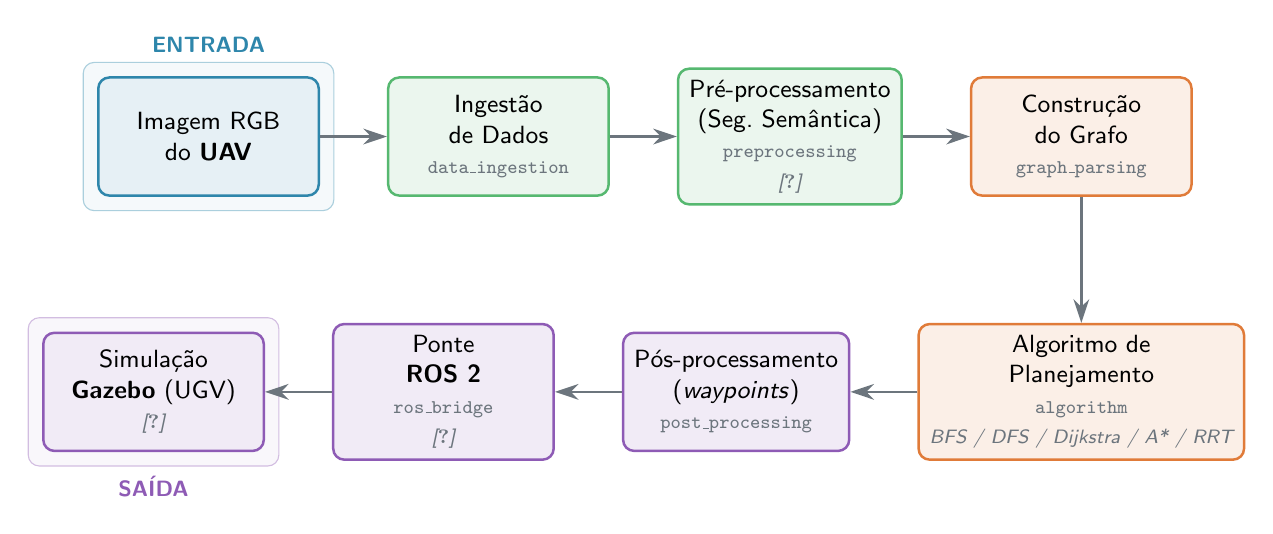
\begin{tikzpicture}[
        node distance=0.85cm and 0.85cm,
        every node/.append style={font=\small\sffamily}
    ]

        \node[pipelineBox=boxBlue]                    (img)
            {Imagem RGB \\ do \textbf{UAV}};
        \node[pipelineBox=boxGreen,  right=of img]    (ingest)
            {Ingestão \\ de Dados \\
             {\scriptsize\color{boxGray}\texttt{data\_ingestion}}};
        \node[pipelineBox=boxGreen,  right=of ingest] (pre)
            {Pré-processamento \\ (Seg.\ Semântica) \\
             {\scriptsize\color{boxGray}\texttt{preprocessing}} \\
             {\scriptsize\itshape\color{boxGray}\cite{junior2024_models}}};
        \node[pipelineBox=boxOrange, right=of pre]    (graph)
            {Construção \\ do Grafo \\
             {\scriptsize\color{boxGray}\texttt{graph\_parsing}}};

        \node[pipelineBox=boxOrange, below=1.6cm of graph] (algo)
            {Algoritmo de \\ Planejamento \\
             {\scriptsize\color{boxGray}\texttt{algorithm}} \\
             {\scriptsize\itshape\color{boxGray}BFS / DFS / Dijkstra / A* / RRT}};
        \node[pipelineBox=boxPurple, left=of algo]    (post)
            {Pós-processamento \\ (\textit{waypoints}) \\
             {\scriptsize\color{boxGray}\texttt{post\_processing}}};
        \node[pipelineBox=boxPurple, left=of post]    (bridge)
            {Ponte \\ \textbf{ROS 2} \\
             {\scriptsize\color{boxGray}\texttt{ros\_bridge}} \\
             {\scriptsize\itshape\color{boxGray}\cite{quigley2009}}};
        \node[pipelineBox=boxPurple, left=of bridge]  (gz)
            {Simulação \\ \textbf{Gazebo} (UGV) \\
             {\scriptsize\itshape\color{boxGray}\cite{koenig2004}}};

        \draw[pipelineArrow] (img)    -- (ingest);
        \draw[pipelineArrow] (ingest) -- (pre);
        \draw[pipelineArrow] (pre)    -- (graph);
        \draw[pipelineArrow] (graph.south) -- (algo.north);
        \draw[pipelineArrow] (algo)   -- (post);
        \draw[pipelineArrow] (post)   -- (bridge);
        \draw[pipelineArrow] (bridge) -- (gz);

        \node[font=\footnotesize\sffamily\bfseries, text=boxBlue,
              anchor=south, above=0.18cm of img.north]
            {ENTRADA};
        \node[font=\footnotesize\sffamily\bfseries, text=boxPurple,
              anchor=north, below=0.18cm of gz.south]
            {SAÍDA};

        \begin{scope}[on background layer]
            \node[draw=boxBlue!40, fill=boxBlue!5, rounded corners=4pt,
                  fit=(img), inner sep=5pt] {};
            \node[draw=boxPurple!40, fill=boxPurple!5, rounded corners=4pt,
                  fit=(gz), inner sep=5pt] {};
        \end{scope}

    \end{tikzpicture}}
    \caption{Pipeline completo do sistema. Em relação à primeira versão (VE), o RRT foi acrescentado ao módulo \texttt{algorithm} e a ponte \texttt{ros\_bridge} foi inserida entre o pós-processamento e a simulação no Gazebo.}
    \label{fig:pipeline}
\end{figure}

\subsection{Diferenças em Relação à Primeira Versão e ao PFC 2025}
\label{subsec:diferencas}

Em relação ao PFC 2025 \cite{camelo2025}, a arquitetura difere principalmente quanto à organização do código e ao acoplamento entre etapas: naquele trabalho, leitura de imagem, segmentação por cor, construção do grafo e execução dos algoritmos eram fortemente acopladas em \textit{scripts} sequenciais, o que tornava trabalhosa a substituição de qualquer uma das etapas. Em relação à primeira versão deste projeto (VE), a diferença não está na organização, que foi mantida, mas no fato de que os módulos de segmentação e de saída deixaram de ser apenas interfaces vazias e passaram a ter implementações completas. A Figura~\ref{fig:comparacao_arquitetura} resume as diferenças.

\begin{figure}[H]
    \centering
    \resizebox{0.95\textwidth}{!}{%
    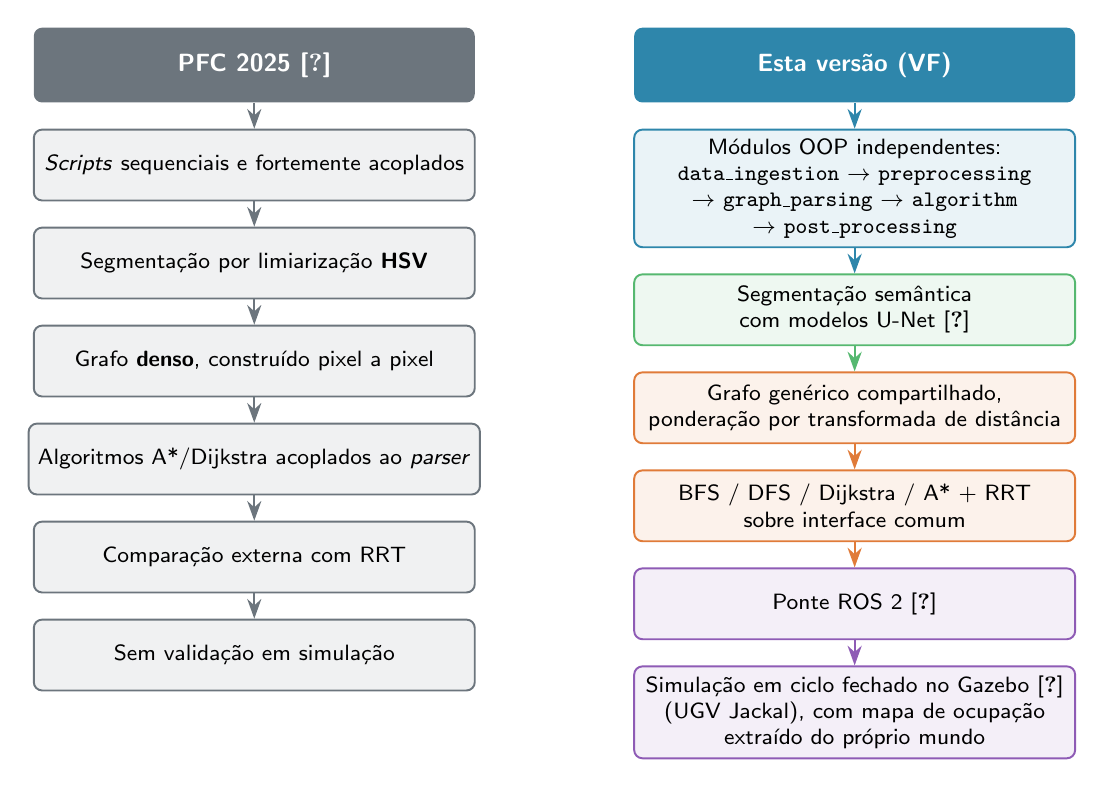
\begin{tikzpicture}[node distance=0.32cm]

        \node[compTitle=boxGray] (tA) {PFC 2025 \cite{camelo2025}};
        \node[compBox=boxGray, below=of tA] (a1)
            {\textit{Scripts} sequenciais e fortemente acoplados};
        \node[compBox=boxGray, below=of a1] (a2)
            {Segmentação por limiarização \textbf{HSV}};
        \node[compBox=boxGray, below=of a2] (a3)
            {Grafo \textbf{denso}, construído pixel a pixel};
        \node[compBox=boxGray, below=of a3] (a4)
            {Algoritmos A*/Dijkstra acoplados ao \textit{parser}};
        \node[compBox=boxGray, below=of a4] (a5)
            {Comparação externa com RRT};
        \node[compBox=boxGray, below=of a5] (a6)
            {Sem validação em simulação};

        \foreach \src/\dst in {tA/a1, a1/a2, a2/a3, a3/a4, a4/a5, a5/a6}{
            \draw[compArrow=boxGray] (\src) -- (\dst);
        }

        \node[compTitle=boxBlue, right=2.0cm of tA] (tB) {Esta versão (VF)};
        \node[compBox=boxBlue, below=of tB] (b1)
            {Módulos OOP independentes:\\
             \texttt{data\_ingestion} $\to$ \texttt{preprocessing}\\
             $\to$ \texttt{graph\_parsing} $\to$ \texttt{algorithm}\\
             $\to$ \texttt{post\_processing}};
        \node[compBox=boxGreen, below=of b1] (b2)
            {Segmentação semântica\\ com modelos U-Net \cite{junior2024_models}};
        \node[compBox=boxOrange, below=of b2] (b3)
            {Grafo genérico compartilhado,\\ ponderação por transformada de distância};
        \node[compBox=boxOrange, below=of b3] (b4)
            {BFS / DFS / Dijkstra / A* + RRT\\ sobre interface comum};
        \node[compBox=boxPurple, below=of b4] (b5)
            {Ponte ROS 2 \cite{quigley2009}};
        \node[compBox=boxPurple, below=of b5] (b6)
            {Simulação em ciclo fechado no Gazebo \cite{koenig2004}\\ (UGV Jackal), com mapa de ocupação\\ extraído do próprio mundo};

        \draw[compArrow=boxBlue]   (tB) -- (b1);
        \draw[compArrow=boxBlue]   (b1) -- (b2);
        \draw[compArrow=boxGreen]  (b2) -- (b3);
        \draw[compArrow=boxOrange] (b3) -- (b4);
        \draw[compArrow=boxOrange] (b4) -- (b5);
        \draw[compArrow=boxPurple] (b5) -- (b6);

    \end{tikzpicture}}
    \caption{Comparativo da estrutura entre o PFC 2025 \cite{camelo2025} e esta versão final. Em destaque, na coluna da direita, os componentes concluídos ao longo deste projeto: segmentação semântica, inclusão do RRT e simulação em ciclo fechado.}
    \label{fig:comparacao_arquitetura}
\end{figure}

% -- 3.2 -------------------------------------------------------------------
\section{Construção dos Grafos}
\label{sec:construcao_grafos}

A construção dos grafos toma como entrada o mapa de navegabilidade gerado pela segmentação (Seção~\ref{sec:mapa_navegabilidade}). O \textit{parser} identifica como nós os pixels marcados como transitáveis e estabelece arestas entre vizinhos imediatos, conforme a conectividade escolhida.

Sobre a definição de grafo $G = (V, E)$ da Seção~2.3, adota-se neste projeto uma representação enriquecida, composta por:

\begin{itemize}
    \item \textbf{\textit{Node embeddings}}: vetor $(x, y, w)$ para cada nó, com as coordenadas espaciais $(x, y)$ do pixel e o peso de transitabilidade $w$;
    \item \textbf{\textit{Edge index}}: tensor de dimensão $(2, |E|)$ com os pares (origem, destino) de cada aresta, seguindo a convenção do PyTorch Geometric;
    \item \textbf{\textit{Edge embeddings}}: vetor $(c_w, d_u)$ para cada aresta, com o custo ponderado $c_w$ e a distância euclidiana $d_u$, definidos a seguir.
\end{itemize}

A escolha dessa representação não é apenas organizacional. Ao separar os atributos dos nós, a lista de arestas e os atributos das arestas em três estruturas numéricas independentes, o grafo fica pronto para ser consumido por bibliotecas de aprendizado em grafos sem conversão adicional, o que deixa aberta a possibilidade de, em trabalhos futuros, aprender a função de custo em vez de defini-la manualmente.

\subsection{Função de Peso e Custo das Arestas}

O peso de transitabilidade e os custos das arestas concretizam a função de pesos $w : E \to \mathbb{R}_{\geq 0}$ introduzida na Seção~\ref{sec:caminhos_minimos}, penalizando trajetórias próximas a obstáculos. Seja $d(v)$ a distância euclidiana de um nó $v$ ao obstáculo mais próximo, obtida pela transformada de distância (\texttt{scipy.ndimage.distance\_transform\_edt}); sejam $r$ (\texttt{robot\_size}) a folga mínima exigida e $L$ (\texttt{weight\_limit}) o raio do campo de proximidade. O peso de um nó é dado por

\[
w(v) =
\begin{cases}
\infty, & \text{se } d(v) \leq r \quad \text{(nó bloqueado)},\\[0.3em]
L - d(v), & \text{se } r < d(v) < L,\\[0.3em]
0, & \text{se } d(v) \geq L.
\end{cases}
\]

A leitura da expressão é a seguinte. Nós a menos de $r$ pixels de um obstáculo são descartados, porque o veículo não caberia ali: $r$ representa, em pixels, o raio do robô mais uma margem de segurança. Entre $r$ e $L$, o peso cresce linearmente à medida que o nó se aproxima do obstáculo, o que torna os caminhos rentes às bordas mais caros sem proibi-los. A partir de $L$ pixels de distância, considera-se que não há mais influência do obstáculo e o peso é nulo. O parâmetro $L$ controla, portanto, o quanto o planejador prefere andar pelo meio dos corredores livres.

Para uma aresta $e = (u, v)$, seja $\delta_{uv} \in \{1, \sqrt{2}\}$ o comprimento do passo, sendo $1$ para vizinhos ortogonais e $\sqrt{2}$ para diagonais. Os dois custos armazenados no \textit{edge embedding} são

\[
d_u = \delta_{uv}, \qquad c_w = \delta_{uv} + w(v),
\]

isto é, $d_u$ é a distância geométrica pura, utilizada na busca não ponderada, e $c_w$ é o custo ponderado, utilizado na busca ponderada, que soma ao comprimento do passo o peso de proximidade do nó de destino. É esse custo $c_w$ que penaliza a proximidade de obstáculos e produz caminhos mais afastados de regiões de risco.

Como consequência dessa definição, o custo total reportado para um caminho ponderado não tem unidade de comprimento: ele mistura pixels percorridos com penalizações de proximidade. Por isso, as tabelas de resultados reportam também a distância percorrida pelo caminho, em pixels, que é a soma dos $d_u$.

\subsection{Eficiência da Construção}

Os principais aprimoramentos em relação ao PFC 2025 \cite{camelo2025} na etapa de construção são:

\begin{itemize}
    \item \textbf{Ponderação por transformada de distância}: o peso de cada nó é obtido em uma única passagem pela imagem com \texttt{scipy.ndimage.distance\_transform\_edt}, substituindo a verificação iterativa pixel a pixel do projeto anterior, na qual, para cada pixel, percorria-se a sua vizinhança em busca de obstáculos;
    \item \textbf{Construção vetorizada}: as arestas são construídas com operações NumPy sobre a matriz inteira, evitando laços Python sobre cada pixel. Em um grafo de alguns milhões de arestas, essa diferença é da ordem de duas ordens de grandeza no tempo de construção.
\end{itemize}

A função \texttt{build\_grid\_graph()}, em \texttt{graph\_parsing/\_grid\_utils.py}, é compartilhada entre o \texttt{GridImageGraphParser}, usado para imagens com cores fixas como o mapa de navegabilidade adotado em \cite{junior2025_rrt}, e o \texttt{SegmentedImageGraphParser}, usado para imagens segmentadas semanticamente.

% -- 3.3 -------------------------------------------------------------------
\section{Inclusão do Algoritmo RRT}
\label{sec:impl_rrt}

O RRT (Seção~\ref{sec:rrt}) foi adicionado ao módulo \texttt{algorithm} sob a mesma interface \texttt{PathAlgorithm} dos demais planejadores, sendo registrado na fábrica ao lado de BFS, DFS, Dijkstra e A*. A implementação segue de perto a referência de Junior \cite{junior2025_rrt}, porém integrada à arquitetura do projeto:

\begin{itemize}
    \item \textbf{Espaço contínuo sobre o mapa.} Ao contrário dos algoritmos de busca em grafos, que operam sobre a estrutura discreta, o RRT opera em coordenadas contínuas de pixel. O espaço livre, as coordenadas de origem e destino e a folga aos obstáculos são obtidos a partir do próprio \texttt{Graph}: um pixel é livre quando é um nó transitável e está suficientemente afastado de obstáculos, ou seja, quando o seu peso é finito segundo a transformada de distância. Assim, o RRT respeita a mesma folga (\texttt{robot\_size}) dos demais algoritmos, o que coloca todos os planejadores nas mesmas condições;
    \item \textbf{Verificação de colisão.} Segue a convenção de \cite{junior2025_rrt}: amostram-se cerca de 100 pontos ao longo do segmento entre duas posições, exigindo-se que todos recaiam sobre o espaço livre. A amostragem é feita de forma paramétrica, o que evita a divisão por zero da implementação de referência em segmentos verticais;
    \item \textbf{Compatibilidade com o pós-processamento.} Cada \textit{waypoint} da árvore é associado ao nó de grafo mais próximo, de modo que os pós-processadores existentes, de geração de \textit{waypoints} e de desenho sobre a imagem, funcionem sem alteração. O custo reportado é o comprimento geométrico do caminho, e não o custo ponderado dos algoritmos de busca;
    \item \textbf{Parâmetros.} \textit{Step size} (padrão 20 px), número máximo de iterações, taxa de amostragem do objetivo e valor inicial do gerador de números aleatórios, este último para permitir reprodutibilidade. São expostos tanto na linha de comando quanto na interface gráfica de teste.
\end{itemize}

% -- 3.4 -------------------------------------------------------------------
\section{Implementação da Segmentação Semântica}
\label{sec:impl_segmentacao}

O módulo \texttt{preprocessing} executa os modelos de \cite{junior2024_models}. Cada modelo é uma rede U-Net \cite{ronneberger2015} com um \textit{backbone} convolucional (ResNet 50/101, EfficientNet-B4/B5 ou MobileNet V2), que produz, para cada pixel, uma distribuição sobre as 23 classes do \emph{Semantic Drone Dataset}. O processamento compreende:

\begin{enumerate}
    \item \textbf{Pré-processamento da imagem.} Conversão para RGB, normalização estatística com a média e o desvio-padrão da ImageNet, coerentes com o treinamento, e, como o codificador reduz a resolução por um fator de 32, preenchimento (\textit{padding}) das bordas até o múltiplo de 32 mais próximo, recortado após a inferência. Sem esse preenchimento, as dimensões da saída do decodificador não coincidem com as da entrada e a rede falha;
    \item \textbf{Inferência e agrupamento de classes.} A classe de cada pixel é obtida pelo índice de maior probabilidade (\textit{argmax}); as classes são então agrupadas em transitável e não transitável, considerando-se transitáveis as classes de solo (\textit{paved-area}, \textit{dirt}, \textit{grass}, \textit{gravel}), segundo critérios herdados de \cite{junior2024};
    \item \textbf{Pós-processamento opcional da máscara.} Filtragem por confiança da predição, redimensionamento e limpeza morfológica, que consiste em fechamento e abertura seguidos da remoção de componentes conexos pequenos. O fechamento preenche buracos internos da máscara, a abertura elimina ruído isolado e a remoção de componentes descarta ilhas transitáveis desconectadas da região principal. Estas etapas são configuráveis e vêm desativadas, de modo que a configuração de origem entregue a máscara bruta do modelo;
    \item \textbf{Geração do mapa de navegabilidade.} Aplicação da paleta de cores de \cite{junior2025_rrt}, produzindo o mapa consumido pelo \texttt{graph\_parsing}.
\end{enumerate}

A seleção do modelo em tempo de execução é um hiperparâmetro do \textit{pipeline}, o que permite trocar o \textit{backbone} sem alterar os demais módulos.

% -- 3.5 -------------------------------------------------------------------
\section{Integração com ROS 2 e Simulação no Gazebo}
\label{sec:ros_integracao}

Esta etapa fecha o ciclo entre planejamento e execução. Ela é composta por dois lados: a publicação a partir do \textit{pipeline} de planejamento e o consumo pelo robô simulado.

\subsection{Publicação: a ponte \texttt{ros\_bridge}}

O módulo \texttt{post\_processing} foi estendido com uma ponte ROS 2 (\texttt{ros\_bridge}) que publica dois tópicos: a imagem aérea anotada com a trajetória (\texttt{sensor\_msgs/Image}) e o caminho como uma sequência de poses (\texttt{nav\_msgs/Path}). Como os \textit{waypoints} são expressos em coordenadas de pixel, a ponte os converte para metros pelas expressões da Seção~\ref{sec:gsd}, aplicando o fator de escala e a inversão do eixo vertical. Utiliza-se a política de QoS \textit{transient local} discutida na Seção~\ref{sec:ros2}, para que o robô receba o caminho mesmo que se conecte após a publicação.

\subsection{Consumo: o pacote \texttt{ugv\_bridge} e o UGV simulado}

Do lado do robô, um pacote ROS 2 (\texttt{ugv\_bridge}) reúne os nós que fazem o UGV simulado percorrer a trajetória:

\begin{itemize}
    \item \texttt{path\_follower\_node}: seguidor de \textit{waypoints} para um robô de tração diferencial, detalhado a seguir;
    \item \texttt{tf\_odom\_bridge\_node}: republica, quando necessário, a transformação de pose (TF) como odometria (\texttt{nav\_msgs/Odometry}), formato esperado pelo seguidor. Esse nó é desnecessário quando o veículo já publica odometria própria, como é o caso do Jackal, e por isso pode ser desativado por parâmetro;
    \item \texttt{image\_monitor\_node}: registra a imagem anotada publicada pela ponte, servindo como verificação de que a informação visual também chegou ao lado do robô.
\end{itemize}

O \texttt{path\_follower\_node} implementa um seguidor de \textit{waypoints} simples. A cada ciclo de controle, ele lê a pose atual $(x, y, \theta)$ da odometria, toma o \textit{waypoint} corrente $(x_t, y_t)$ e calcula o erro de proa
\[
e_\theta = \mathrm{atan2}\big(\sin(\theta_d - \theta),\ \cos(\theta_d - \theta)\big),
\qquad
\theta_d = \mathrm{atan2}(y_t - y,\ x_t - x),
\]
onde a forma com seno e cosseno garante que o erro fique no intervalo $(-\pi, \pi]$, evitando que o robô gire pelo lado mais longo. Os comandos publicados em \texttt{geometry\_msgs/Twist} são
\[
\omega = \mathrm{sat}\big(2\,e_\theta,\ \omega_{\max}\big),
\qquad
v = v_{\text{cruzeiro}} \cdot \max\left(0,\ 1 - \frac{|e_\theta|}{\pi/2}\right),
\]
isto é, a velocidade angular é proporcional ao erro de proa, limitada a um valor máximo, e a velocidade linear é reduzida proporcionalmente ao desalinhamento, anulando-se quando o robô precisa girar mais de noventa graus. Esse acoplamento evita que o veículo avance na direção errada enquanto ainda está se alinhando. Um \textit{waypoint} é considerado alcançado quando a distância até ele fica abaixo de uma tolerância, mais folgada para os pontos intermediários e mais apertada para o ponto final.

Como plataforma de demonstração, adotou-se o UGV Clearpath Jackal simulado no Gazebo, iniciado por um \textit{launch file} de integração que sobe a simulação e os nós do \texttt{ugv\_bridge}. Nessa configuração, a odometria filtrada é fornecida por um filtro de Kalman estendido (EKF) que funde a odometria das rodas e a unidade inercial. O fluxo completo é, portanto: o \textit{pipeline} planeja e publica o caminho, o \texttt{path\_follower\_node} converte o caminho em comandos de velocidade, e o Jackal percorre a trajetória no Gazebo até o destino.

A Figura~\ref{fig:gazebo_jackal} mostra o veículo simulado no mundo \textit{warehouse}, com o painel de teleoperação publicando no mesmo tópico de comando de velocidade usado pela integração.

\begin{figure}[H]
    \centering
    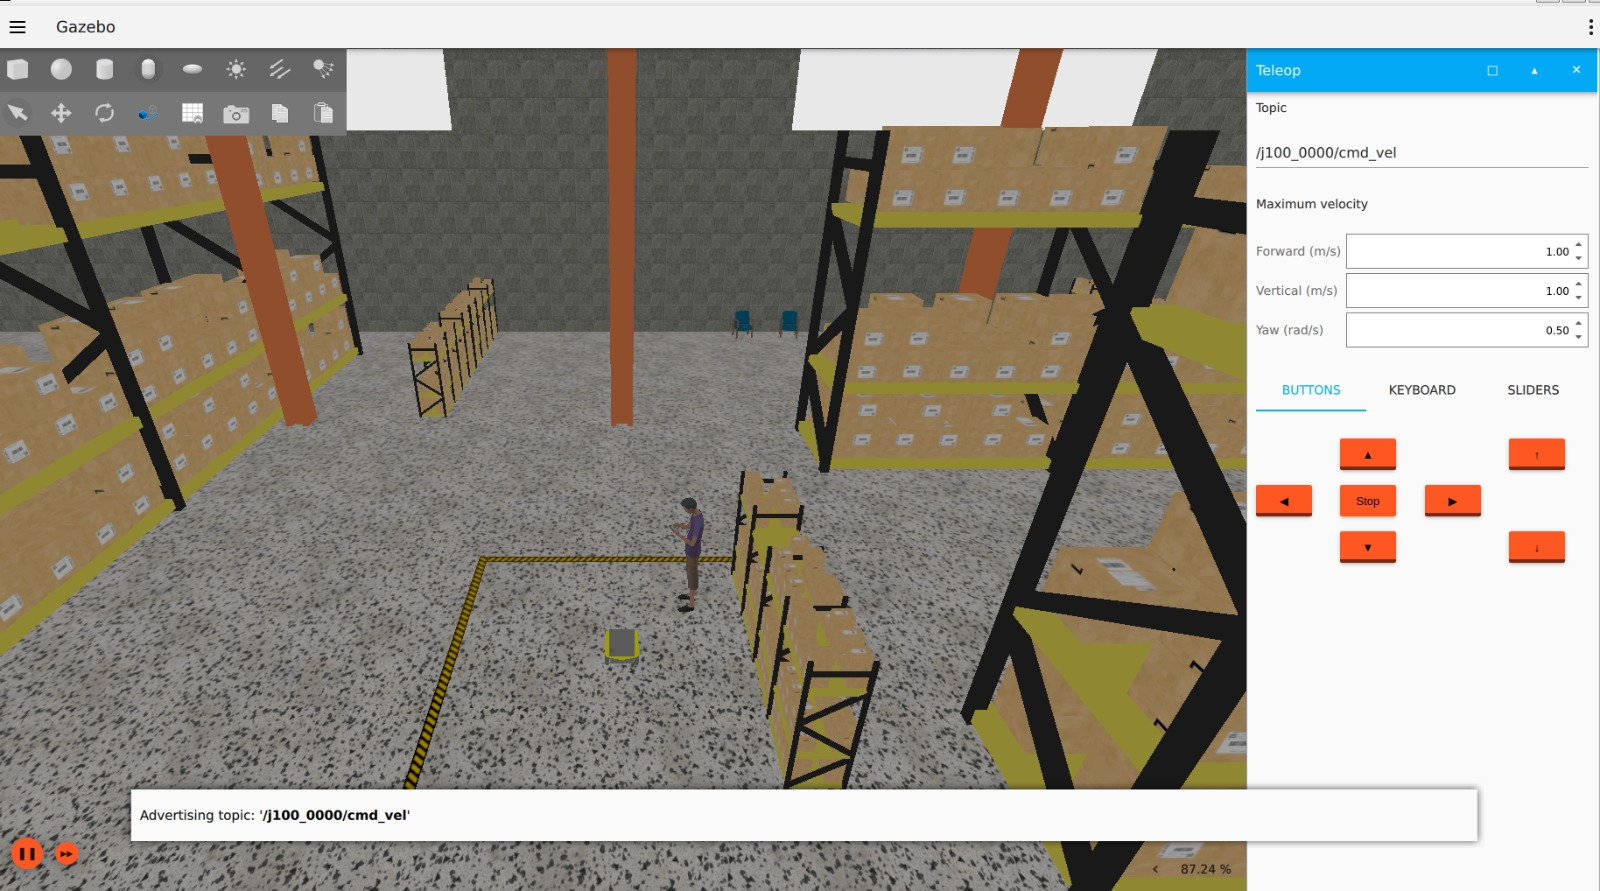
\includegraphics[width=0.95\textwidth]{figuras/gazebo_jackal.jpg}
    \caption{UGV Clearpath Jackal simulado no mundo \textit{warehouse} do Gazebo. À direita, o painel de teleoperação publicando comandos de velocidade (\texttt{geometry\_msgs/Twist}) no tópico \texttt{cmd\_vel} consumido pela integração.}
    \label{fig:gazebo_jackal}
\end{figure}

% -- 3.6 -------------------------------------------------------------------
\section{Geração do Mapa de Ocupação a partir do Mundo Simulado}
\label{sec:mapa_ocupacao}

Esta seção descreve o acréscimo próprio desta versão final.

Na segunda versão (VC), o caminho era planejado sobre uma imagem aérea e depois publicado para o robô no Gazebo. Isso deixava em aberto uma questão de referencial: a imagem aérea e o mundo simulado são cenários distintos, de modo que a correspondência entre eles dependia inteiramente do ajuste manual do fator de escala e da origem. Quando esses valores não eram exatos, o robô percorria uma trajetória com a forma correta, mas deslocada ou fora de escala em relação aos obstáculos do mundo, conforme discutido na Seção~\ref{sec:res_gazebo}.

Para eliminar essa fonte de erro, foi desenvolvido um conversor (\texttt{scripts/\allowbreak gazebo\_\allowbreak world\_\allowbreak to\_\allowbreak occupancy.py}) que lê o arquivo SDF do mundo do Gazebo e produz uma vista superior bidimensional dele, no mesmo formato de mapa de navegabilidade consumido pelo \texttt{graph\_parsing} (Seção~\ref{sec:mapa_navegabilidade}). O procedimento é:

\begin{enumerate}
    \item \textbf{Percurso da árvore do mundo.} São visitados todos os modelos definidos diretamente no arquivo e todos os modelos incluídos por referência, resolvidos tanto em diretórios locais quanto no cache de modelos baixados do repositório de modelos do simulador;
    \item \textbf{Composição de poses.} Cada elemento de colisão tem a sua pose composta com as poses do elo (\textit{link}) e do modelo que o contêm, resultando em uma transformação homogênea que leva a geometria local para o referencial do mundo;
    \item \textbf{Rasterização da geometria.} Caixas e cilindros são projetados diretamente no plano horizontal. Malhas trianguladas no formato STL têm seus triângulos transformados e projetados; triângulos quase horizontais, que correspondem a pisos e tetos, são descartados por um critério de inclinação, de modo que apenas geometria de parede se torne obstáculo. Elementos que não podem ser resolvidos, como planos infinitos ou malhas em formatos não suportados, são ignorados com aviso, e não viram obstáculo;
    \item \textbf{Escrita do mapa.} A área livre recebe a cor transitável convencionada e os obstáculos recebem preto. O programa imprime os valores exatos de resolução em metros por pixel e de origem em metros a serem passados ao \textit{pipeline}, de forma que o caminho planejado caia exatamente sobre o referencial do mundo.
\end{enumerate}

O resultado, para o mundo \textit{warehouse}, é mostrado na Figura~\ref{fig:mapa_ocupacao}. A consequência prática é que o planejamento passa a ocorrer sobre a geometria real do ambiente em que o veículo vai se mover, com correspondência métrica exata, o que separa claramente dois tipos de erro que antes se confundiam: erros do planejador e erros de alinhamento entre referenciais.

\begin{figure}[H]
    \centering
    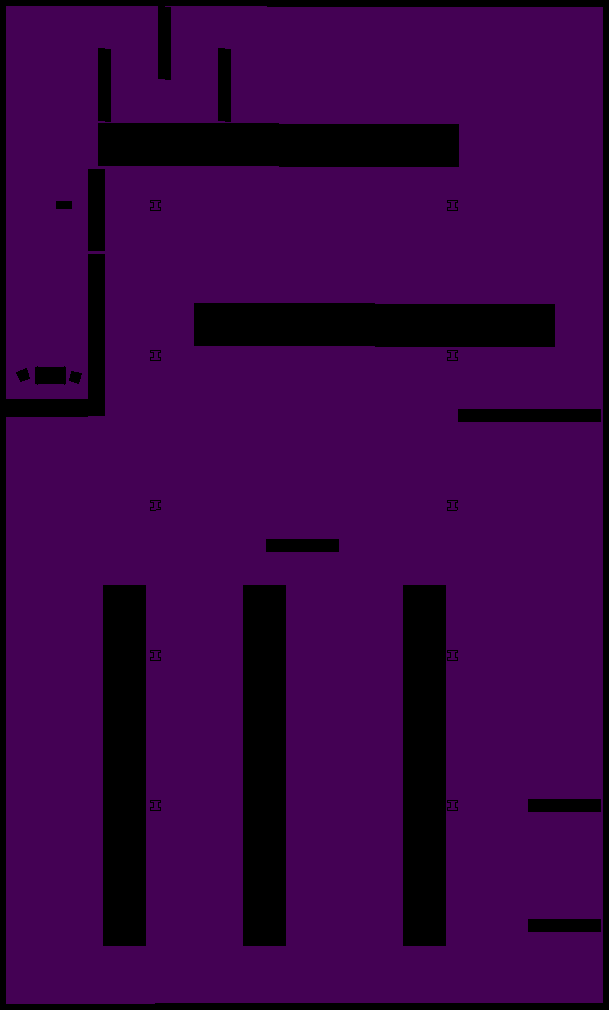
\includegraphics[width=0.52\textwidth]{figuras/mapa_ocupacao.png}
    \caption{Mapa de ocupação gerado automaticamente a partir da descrição SDF do mundo \textit{warehouse} do Gazebo. Em roxo, a área livre, na cor convencionada para regiões transitáveis; em preto, a geometria de colisão projetada no plano horizontal. Resolução de 0,05 m por pixel.}
    \label{fig:mapa_ocupacao}
\end{figure}

% -- 3.7 -------------------------------------------------------------------
\section{Pós-processamento e Formato de Saída}

Além da ponte ROS 2, o módulo \texttt{post\_processing} mantém dois processadores. O \texttt{SimpleWaypointProcessor} converte a sequência de nós em \textit{waypoints} com coordenadas $(x, y)$, ângulo de proa $\theta$ e tipo de movimento, encapsulados na \textit{dataclass} \texttt{RobotPath}. O ângulo de proa de cada ponto é o da direção para o ponto seguinte, o que dá ao seguidor uma referência de orientação além da posição. O \texttt{ImageDrawingPostProcessor} desenha os caminhos sobre a imagem original, com cores distintas por algoritmo e marcadores de início e fim, e é a origem das figuras comparativas do Capítulo~\ref{cap:resultados}.

% -- 3.8 -------------------------------------------------------------------
\section{Coleta dos Dados e Ambiente Experimental}
\label{sec:ambiente}

Para os experimentos, são utilizadas imagens RGB de alta resolução obtidas por drone, em cenários representativos de operação do UGV, com caminhos pavimentados, vegetação, praças e obstáculos diversos, incluindo imagens da Quinta da Boa Vista e de área urbana adensada. Os modelos de segmentação adotados já foram treinados em \cite{junior2024_models} sobre o \emph{Semantic Drone Dataset} \cite{drone_dataset} e são aqui avaliados sobre essas imagens reais, ou seja, em cenários diferentes daqueles em que foram treinados. Além das imagens aéreas, utiliza-se o mapa de ocupação do mundo \textit{warehouse}, gerado conforme a Seção~\ref{sec:mapa_ocupacao}.

Os ensaios de segmentação e de planejamento foram executados em duas máquinas. Os resultados de segmentação da Seção~\ref{sec:res_segmentacao} foram obtidos com aceleração em GPU integrada de arquitetura Apple Silicon. Os resultados de planejamento da Seção~\ref{sec:res_algoritmos} sobre o mapa de ocupação foram obtidos em processador Intel Core i7-1265U com 16 GB de memória, sem uso de GPU, uma vez que essa etapa não envolve inferência de rede neural. A simulação foi executada em ROS 2 Humble e Gazebo sobre Ubuntu 22.04 em WSL2, configuração cujas limitações são discutidas na Seção~\ref{sec:limitacoes}.

% ======================================================================
\chapter{RESULTADOS E DISCUSSÃO}
\label{cap:resultados}
% ======================================================================

Neste capítulo, apresentamos e discutimos os resultados obtidos. As três primeiras seções tratam, respectivamente, dos modelos de segmentação, dos algoritmos de planejamento e da execução da trajetória no simulador. A última seção reúne as limitações encontradas e as dificuldades que impediram o cumprimento integral do cronograma.

% -- 4.1 -------------------------------------------------------------------
\section{Comparação dos Modelos de Segmentação}
\label{sec:res_segmentacao}

A Tabela~\ref{tab:comparacao_modelos} reúne, para os modelos com métricas publicadas em \cite{junior2024_models}, a mIoU e a acurácia no conjunto de teste do \emph{Semantic Drone Dataset}, além da fração de área classificada como transitável e do tempo de inferência medidos neste trabalho sobre uma imagem representativa redimensionada para $1024 \times 768$ pixels. A implementação suporta ainda o \textit{backbone} MobileNet V2, aqui omitido da comparação quantitativa por não haver métricas de referência publicadas.

\begin{table}[H]
    \centering
    \caption{Comparação dos modelos de segmentação. As colunas mIoU e acurácia são as publicadas em \cite{junior2024_models}; a área transitável e o tempo de inferência foram medidos neste trabalho, sobre imagem de $1024 \times 768$ pixels, com aceleração em GPU integrada.}
    \label{tab:comparacao_modelos}
    \begin{tabular}{lcccc}
        \toprule
        \textbf{Modelo} & \textbf{mIoU} & \textbf{Acurácia} & \textbf{Área transit.\ (\%)} & \textbf{Tempo (s)} \\
        \midrule
        ResNet~50        & 0,3933 & 0,8244 & 65,5 & 0,72 \\
        ResNet~101       & 0,4032 & 0,8720 & 67,5 & 0,52 \\
        EfficientNet-B4  & 0,5012 & 0,9120 & 61,1 & 0,71 \\
        EfficientNet-B5  & 0,4819 & 0,9025 & 69,4 & 0,57 \\
        \bottomrule
    \end{tabular}
\end{table}

Os modelos EfficientNet apresentam as melhores métricas de referência, com destaque para o EfficientNet-B4, de maior mIoU (0,5012). Os tempos de inferência são todos inferiores a um segundo na resolução avaliada, sem diferença expressiva entre os \textit{backbones}, o que torna a mIoU o principal critério de escolha.

A coluna de área transitável merece um comentário, porque é a única medida obtida sobre as imagens deste trabalho e não sobre o conjunto de teste do \emph{Semantic Drone Dataset}. Ela indica a fração da imagem que cada modelo considerou navegável. Não existe um valor correto conhecido para essas imagens, já que elas não são anotadas, mas a dispersão entre os modelos, de 61,1\% a 69,4\%, mostra que a escolha do \textit{backbone} altera de forma perceptível o espaço livre entregue ao planejador. Um modelo mais permissivo produz um grafo maior e pode incluir como transitáveis regiões de risco; um modelo mais conservador reduz o espaço de busca e pode fechar corredores estreitos. Nota-se que o EfficientNet-B4, de maior mIoU, é também o mais conservador dos quatro, o que é coerente com uma segmentação mais criteriosa das bordas entre classes.

A Figura~\ref{fig:segmentacao} mostra, para o EfficientNet-B4, a máscara de área transitável sobreposta à imagem de entrada. O pátio pavimentado e a vegetação rasteira são corretamente identificados como transitáveis, ao passo que o coreto, as edificações, as árvores densas e os veículos são excluídos. As bordas acompanham os limites reais das estruturas, inclusive em regiões sombreadas, o que era justamente a dificuldade das abordagens por limiarização de cor usadas no PFC 2025.

\begin{figure}[H]
    \centering
    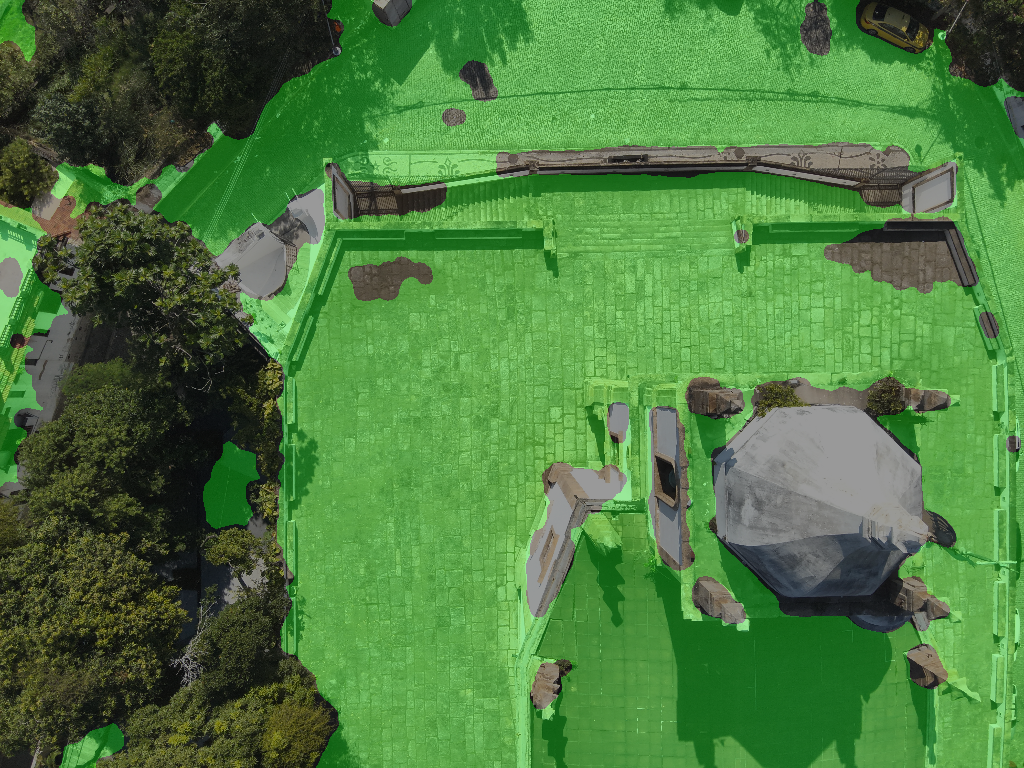
\includegraphics[width=0.95\textwidth]{figuras/segmentacao_b4.png}
    \caption{Segmentação com o modelo EfficientNet-B4: em verde, a região classificada como transitável, sobreposta à imagem aérea de entrada.}
    \label{fig:segmentacao}
\end{figure}

% -- 4.2 -------------------------------------------------------------------
\section{Desempenho dos Algoritmos de Planejamento}
\label{sec:res_algoritmos}

\subsection{Comparação sobre Imagem Aérea Segmentada}

A Tabela~\ref{tab:comparacao_algoritmos} compara os cinco algoritmos sobre o mesmo grafo, gerado a partir de uma imagem aérea redimensionada para $1000 \times 750$ pixels, com cerca de $4{,}4 \times 10^5$ nós e $3{,}3 \times 10^6$ arestas, e com os mesmos pontos de origem e destino. Para os algoritmos de busca, o custo reportado é o custo ponderado $c_w$, que penaliza a proximidade de obstáculos conforme a ponderação definida na Seção~\ref{sec:construcao_grafos}; para o RRT, é o comprimento geométrico do caminho.

\begin{table}[H]
    \centering
    \caption{Comparação dos algoritmos sobre o mesmo mapa ($1000 \times 750$ pixels; mesmos pontos de início e fim). Na coluna Custo, o valor do RRT é o comprimento geométrico do caminho, que não é comparável ao custo ponderado dos demais algoritmos. A quarta coluna traz o número de nós explorados pelos algoritmos de busca e o número de iterações do RRT.}
    \label{tab:comparacao_algoritmos}
    \small
    \setlength{\tabcolsep}{5pt}
    \begin{tabular}{lrrrrr}
        \toprule
        \textbf{Algoritmo}
            & \shortstack[r]{\textbf{Nós do}\\\textbf{caminho}}
            & \textbf{Custo}
            & \shortstack[r]{\textbf{Nós expl.}\\\textbf{ou iter.}}
            & \shortstack[r]{\textbf{Tempo}\\\textbf{(s)}}
            & \shortstack[r]{\textbf{Distância}\\\textbf{(px)}} \\
        \midrule
        BFS      &    351 &    12.838,8 & 179.546 & 0,131 &    398,0 \\
        DFS      & 65.282 & 1.314.372,7 & 248.479 & 0,159 & 92.241,7 \\
        Dijkstra &    879 &     1.462,2 & 228.525 & 0,392 &    990,7 \\
        A*       &    879 &     1.462,2 & 203.472 & 0,426 &    990,7 \\
        RRT      &     30 &       931,6 &     289 & 0,010 &    931,8 \\
        \bottomrule
    \end{tabular}
\end{table}

Os resultados são coerentes com a teoria e com o observado no PFC 2025 \cite{camelo2025}:

\begin{itemize}
    \item \textbf{A* e Dijkstra} produzem exatamente o mesmo caminho ótimo ponderado, de custo 1.462,2, mas o A* explora menos nós, 203.472 contra 228.525, graças à heurística, o que confirma a preferência pelo A* já apontada no PFC 2025. Vale notar que, mesmo explorando cerca de 11\% menos nós, o A* não foi mais rápido em tempo de execução neste ensaio, pelo motivo discutido na Seção~\ref{sec:caminhos_minimos}: o custo por nó expandido é maior, porque cada vizinho exige o cálculo da heurística euclidiana. A vantagem do A* cresce quando o grafo é maior ou quando a heurística é mais informativa em relação ao formato do espaço livre;
    \item \textbf{A BFS} encontra o caminho com menor número de arestas, o que corresponde à menor distância percorrida, de 398,0 px, porém, por ignorar os pesos, apresenta o maior custo ponderado entre os algoritmos ótimos, de 12.838,8. Esse par de valores mostra com clareza a diferença entre os dois critérios: o caminho mais curto passa rente aos obstáculos, e o caminho de menor custo ponderado aceita ser cerca de duas vezes e meia mais longo em troca de manter distância deles;
    \item \textbf{A DFS} confirma seu caráter não ótimo, produzindo um caminho de 65.282 nós, com distância percorrida duas ordens de grandeza maior que a dos demais. Ela percorre quase toda a região transitável antes de alcançar o destino, e é mantida na comparação apenas como referência do que acontece quando não há nenhum critério de custo;
    \item \textbf{O RRT} é o mais rápido por larga margem, com 0,010 s e apenas 289 iterações, e produz um caminho curto em comprimento geométrico, porém irregular e não ótimo, além de sujeito à variabilidade estocástica entre execuções.
\end{itemize}

A Figura~\ref{fig:caminhos_aerea} mostra os caminhos produzidos sobre uma imagem aérea de área urbana adensada, na qual a região amarela corresponde ao que a segmentação classificou como não transitável. O marcador vermelho indica o ponto de partida e o verde o de chegada. A figura ilustra, de forma visual, três pontos discutidos acima.

\begin{figure}[H]
    \centering
    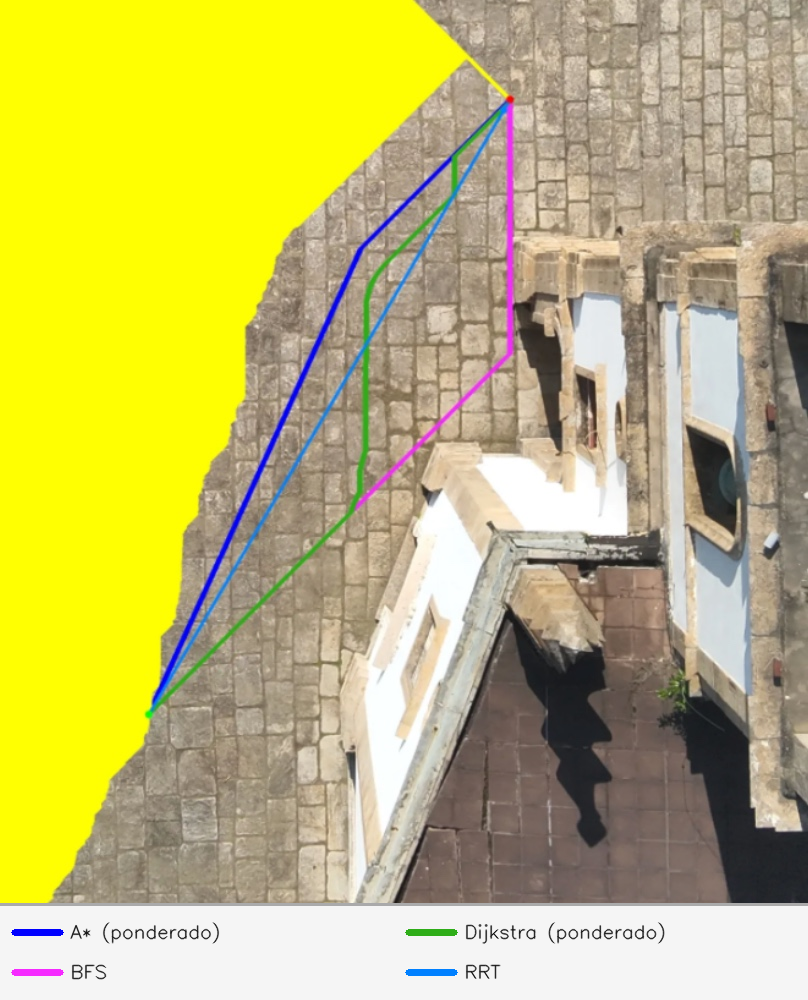
\includegraphics[width=0.66\textwidth]{figuras/caminhos_aerea.png}
    \caption{Caminhos calculados pelos diferentes algoritmos sobre imagem aérea de área urbana. Em amarelo, a região classificada como não transitável; marcador vermelho no ponto de partida e verde no de chegada. As cores dos traços seguem a convenção do módulo de pós-processamento, reproduzida na legenda.}
    \label{fig:caminhos_aerea}
\end{figure}

O primeiro ponto é que a BFS, em magenta, contorna o obstáculo pelo trajeto com menor número de passos, o que a leva a acompanhar de perto a borda da região não transitável e a descrever um ângulo acentuado, sem qualquer consideração de segurança. O segundo é que o A* e o Dijkstra, em azul e verde, produzem caminhos distintos apesar de terem o mesmo custo ponderado: em um grafo em grade com pesos idênticos em regiões amplas, há muitos caminhos de custo mínimo, e a ordem de expansão de cada algoritmo determina qual deles é registrado, conforme antecipado na Seção~\ref{sec:caminhos_minimos}. Os dois estão corretos. O terceiro é o comportamento do RRT, em azul claro: o seu traçado não é um caminho da grade, e sim uma cadeia de poucos segmentos retos que ligam pontos amostrados ao acaso, marcados pelos pequenos círculos ao longo da linha. Nesta cena, quase toda a faixa entre origem e destino é livre, e o viés para o objetivo faz o RRT convergir quase em linha reta com apenas 30 nós, contra os 879 dos algoritmos de busca.

\subsection{Comparação sobre o Mapa de Ocupação do Mundo Simulado}

A comparação anterior foi repetida sobre o mapa de ocupação do mundo \textit{warehouse}, gerado conforme a Seção~\ref{sec:mapa_ocupacao}. Esse cenário é mais exigente do que a cena aérea aberta: há prateleiras longas e paralelas, corredores estreitos e paredes internas, de modo que o espaço livre entre origem e destino não é um corredor único e amplo. O grafo resultante tem 502.833 nós e 3.753.214 arestas, a partir de uma imagem de $863 \times 1242$ pixels com resolução de 0,05 m por pixel. Os resultados estão na Tabela~\ref{tab:comparacao_warehouse} e os caminhos correspondentes na Figura~\ref{fig:caminhos_warehouse}.

\begin{table}[H]
    \centering
    \caption{Comparação dos algoritmos sobre o mapa de ocupação do mundo \textit{warehouse} ($863 \times 1242$ pixels, 502.833 nós e 3.753.214 arestas; mesmos pontos de início e fim). Valem aqui as mesmas observações da Tabela~\ref{tab:comparacao_algoritmos} quanto à coluna Custo e à contagem de nós explorados.}
    \label{tab:comparacao_warehouse}
    \small
    \setlength{\tabcolsep}{5pt}
    \begin{tabular}{lrrrrr}
        \toprule
        \textbf{Algoritmo}
            & \shortstack[r]{\textbf{Nós do}\\\textbf{caminho}}
            & \textbf{Custo}
            & \shortstack[r]{\textbf{Nós expl.}\\\textbf{ou iter.}}
            & \shortstack[r]{\textbf{Tempo}\\\textbf{(s)}}
            & \shortstack[r]{\textbf{Distância}\\\textbf{(px)}} \\
        \midrule
        A* (ponderado)       & 610 & 28.676,8 & 391.268 & 2,232 & 709,7 \\
        Dijkstra (ponderado) & 610 & 28.676,8 & 397.683 & 1,587 & 709,7 \\
        BFS                  & 598 & 44.129,0 & 414.573 & 0,677 & 720,9 \\
        RRT                  &  22 &    756,7 &     286 & 0,075 & 755,7 \\
        \bottomrule
    \end{tabular}
\end{table}

\begin{figure}[H]
    \centering
    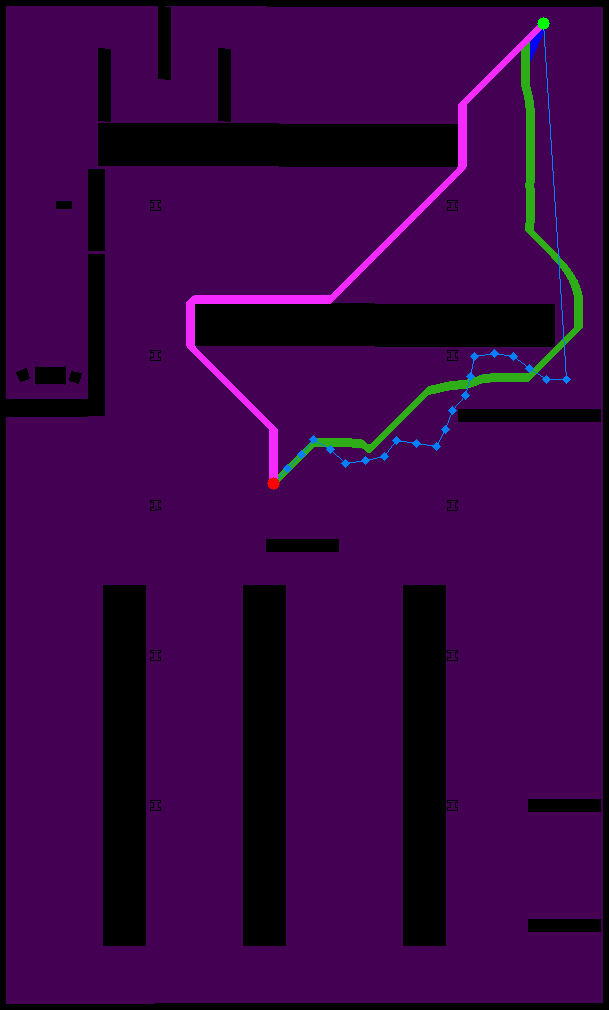
\includegraphics[width=0.56\textwidth]{figuras/caminhos_warehouse.png}
    \caption{Caminhos calculados sobre o mapa de ocupação do mundo \textit{warehouse}. Em verde, o caminho do Dijkstra ponderado, que coincide com o do A* e o encobre no desenho; em magenta, o da BFS; em azul claro, o do RRT. Marcador vermelho no ponto de partida e verde no de chegada.}
    \label{fig:caminhos_warehouse}
\end{figure}

Neste cenário, o A* e o Dijkstra devolveram o mesmo caminho, de 610 nós e custo 28.676,8, que aparece em verde na figura porque o traço do Dijkstra é desenhado por último e cobre o do A*. O A* novamente explorou menos nós que o Dijkstra, ainda que por margem pequena, e novamente levou mais tempo de execução, pelo motivo já discutido. A BFS encontrou um caminho com menos nós e custo ponderado 54\% maior, seguindo um trajeto completamente distinto, que sobe pelo lado esquerdo do galpão.

O comportamento do RRT é o mais informativo desta figura. Com apenas 22 pontos e 286 iterações, ele produziu um caminho com comprimento geométrico próximo ao dos demais, 755,7 px contra 709,7 px, mas com forma visivelmente diferente: enquanto os caminhos determinísticos descrevem curvas suaves e regulares, que acompanham a geometria dos corredores, o traçado do RRT é uma sucessão de segmentos com mudanças bruscas de direção, avançando ora para um lado, ora para o outro, sem relação com a disposição dos obstáculos. Esses desvios são consequência direta do mecanismo do algoritmo, descrito na Seção~\ref{sec:rrt}: cada nó novo é gerado na direção de um ponto amostrado ao acaso, e não na direção do destino, de modo que o caminho reproduz a irregularidade dessa amostragem. Comparando as duas figuras, fica claro que a intensidade desses desvios depende do cenário: na cena aérea aberta da Figura~\ref{fig:caminhos_aerea}, o viés para o objetivo mantém o traçado quase reto; no galpão da Figura~\ref{fig:caminhos_warehouse}, com obstáculos distribuídos ao longo do percurso, o mesmo algoritmo produz desvios pronunciados.

Essa diferença de forma tem consequência prática para um veículo de tração diferencial. Cada mudança brusca de direção obriga o robô a reduzir a velocidade linear e girar, conforme a lei de controle da Seção~\ref{sec:ros_integracao}. Um caminho geometricamente curto, porém com muitos desvios, pode levar mais tempo para ser percorrido do que um caminho um pouco mais longo e suave. Por esse motivo, e apesar do tempo de planejamento muito menor, o RRT não foi adotado como planejador padrão para os ensaios de simulação, nos quais se utilizou o A* ponderado.

% -- 4.3 -------------------------------------------------------------------
\section{Validação no Simulador Gazebo}
\label{sec:res_gazebo}

A integração descrita na Seção~\ref{sec:ros_integracao} foi verificada em execução completa. A partir do \textit{pipeline}, a trajetória planejada é publicada nos tópicos ROS 2 e o UGV Clearpath Jackal simulado no Gazebo a percorre efetivamente, seguindo os \textit{waypoints} por meio do \texttt{path\_follower\_node} até alcançar o ponto de destino, momento em que o nó registra a conclusão do percurso e publica comando de parada.

\subsection{Percursos Executados}

Foram realizados três conjuntos de ensaios, todos concluídos com o robô alcançando o destino:

\begin{enumerate}
    \item \textbf{Percurso de referência em mapa sintético.} Um caminho de 281 \textit{waypoints}, correspondente a cerca de 20 m no referencial do mundo com resolução de 0,05 m por pixel, foi percorrido integralmente em 93,9 s. Durante o percurso foram registradas 4.601 amostras de odometria, o que corresponde a uma taxa média em torno de 49 amostras por segundo. A velocidade média resultante, de aproximadamente 0,21 m/s, é pouco mais da metade da velocidade de cruzeiro configurada, de 0,4 m/s. Essa diferença é explicada pela redução de velocidade linear imposta pela lei de controle durante as correções de proa, e é uma medida indireta de quanto tempo o veículo passou girando em vez de avançando;
    \item \textbf{Percurso sobre imagem aérea real.} A mesma integração foi executada com o caminho planejado diretamente sobre uma imagem de drone de área urbana, com duração de 232,9 s. A Figura~\ref{fig:execucao_dji} mostra o percurso já concluído, com o veículo sobre o ponto de destino;
    \item \textbf{Percurso no mundo \textit{warehouse}.} O percurso mais longo, de 477,6 s, foi executado sobre o mundo simulado, usando o mapa de ocupação da Seção~\ref{sec:mapa_ocupacao}.
\end{enumerate}

\begin{figure}[H]
    \centering
    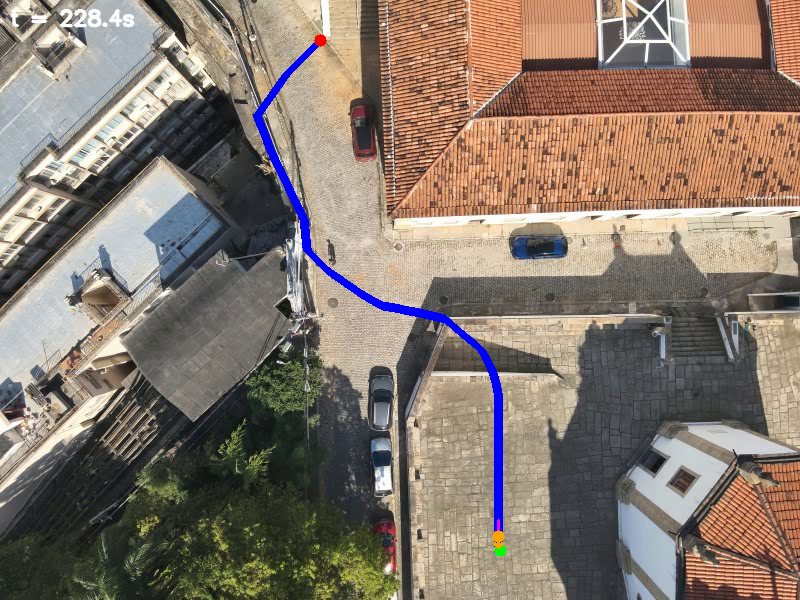
\includegraphics[width=0.85\textwidth]{figuras/execucao_dji.png}
    \caption{Execução do percurso sobre imagem aérea real, no instante $t = 228{,}4$ s, próximo ao final do trajeto. Em azul, o caminho planejado pelo \textit{pipeline}; em vermelho e verde, os pontos de partida e de chegada; em laranja, a posição do UGV simulado, já sobre o ponto de destino, com o rastro recente da odometria em magenta.}
    \label{fig:execucao_dji}
\end{figure}

\subsection{Aderência entre a Trajetória Planejada e a Executada}

A sobreposição do rastro de odometria ao caminho planejado, visível na Figura~\ref{fig:execucao_dji}, mostra que o veículo segue o traçado planejado ao longo de todo o percurso. Os desvios observados concentram-se nas mudanças de direção, onde o veículo descreve uma curva de raio finito enquanto o caminho planejado tem um vértice, e são compatíveis com a tolerância de \textit{waypoint} configurada, de 0,12 m. Nos trechos retos, o rastro é indistinguível do caminho planejado na escala da figura.

Cabe registrar que essa avaliação é geométrica e visual. Uma métrica numérica de erro lateral médio entre a trajetória executada e a planejada não foi calculada, porque exigiria o registro sincronizado da odometria e do caminho em um mesmo referencial, com tratamento do atraso entre as duas fontes. Esse cálculo é direto a partir dos dados já registrados pelo gravador de trajetórias e fica indicado como continuidade imediata.

\subsection{Alinhamento entre Referenciais}

O ponto que mais influenciou o resultado da simulação não foi o planejamento, e sim a correspondência entre o referencial da imagem e o do mundo, discutida na Seção~\ref{sec:gsd}. O veículo é criado no mundo simulado na origem, ao passo que o caminho planejado começa no pixel escolhido pelo operador, que corresponde a outro ponto do mundo. Sem correção, o seguidor interpreta o primeiro \textit{waypoint} como um destino a alcançar e o robô dirige-se até lá antes de iniciar o percurso propriamente dito. Quando a origem informada está errada, esse trecho inicial pode sair inteiramente da área representada pelo mapa, e o percurso registrado parece extrapolar os limites do ambiente.

Duas soluções foram implementadas e verificadas. A primeira é informar corretamente a origem em metros, o que o conversor de mundos da Seção~\ref{sec:mapa_ocupacao} passou a calcular automaticamente para o caso do Gazebo. A segunda é reposicionar o veículo no primeiro \textit{waypoint} antes do início do percurso, recurso disponível por parâmetro no seguidor, com a devida composição da transformação entre os referenciais de odometria e de mundo, para que a estimativa de pose permaneça coerente após o reposicionamento. A primeira solução é a correta para uso realista; a segunda é útil para isolar a avaliação do seguidor da questão de alinhamento.

Do ponto de vista de dados, o simulador recebe como entrada o modelo do robô e do mundo, com geometria, dinâmica e sensores, e os comandos de velocidade gerados pelo seguidor; como saída, publica o estado simulado do veículo, em especial a odometria e as transformações de referencial, além dos fluxos de sensores. É essa odometria que realimenta o \texttt{path\_follower\_node}, fechando a malha de controle.

% -- 4.4 -------------------------------------------------------------------
\section{Limitações e Dificuldades Encontradas}
\label{sec:limitacoes}

Esta seção reúne as limitações do trabalho e as dificuldades que determinaram o seu estágio final, em particular a não realização dos ensaios em ambiente real.

\subsection{Ausência de Validação em Ambiente Real}

O cronograma do projeto previa, para os dois últimos meses, a repetição dos ensaios de simulação em um veículo físico. Essa etapa não foi realizada. As razões são de três naturezas.

A primeira é de \textbf{disponibilidade de plataforma}. Os ensaios de simulação foram conduzidos sobre o modelo do Clearpath Jackal, escolhido por ser uma plataforma de tração diferencial com modelo bem mantido e integração madura com o ROS 2. A transposição para um veículo físico exigiria um UGV com odometria confiável, unidade inercial e interface ROS 2 disponível para uso continuado durante o período de ensaios, condição que não foi possível assegurar dentro do prazo do projeto.

A segunda é de \textbf{espaço e de aquisição de imagem}. O método proposto depende de uma imagem aérea da mesma área em que o veículo vai operar, capturada com a câmera próxima da vertical e com escala conhecida. Isso significa que um ensaio real não se restringe a posicionar o robô em um corredor: é necessário um espaço aberto, com obstáculos permanentes e área livre suficiente para percursos de algumas dezenas de metros, e um voo de UAV sobre esse espaço, com autorização, condições meteorológicas adequadas e medição de referência para determinação do fator de escala em metros por pixel. A coordenação dessas condições, somada à necessidade de repetir o voo caso a imagem não ficasse adequada, tornou o ensaio real incompatível com o prazo remanescente.

A terceira é de \textbf{tempo}. A integração com o ROS 2 e a simulação, prevista para ser uma etapa intermediária, consumiu parcela significativa do cronograma. A depuração da comunicação entre os nós, o tratamento das políticas de QoS, a configuração do \textit{workspace} do simulador e, principalmente, os problemas de ambiente gráfico descritos a seguir ocuparam o período que estava reservado para a transição ao ambiente real.

Convém precisar o alcance dessa ausência. Todo o encadeamento entre o planejamento e o controle do veículo, isto é, a publicação do caminho, o seguimento de \textit{waypoints}, a realimentação por odometria e a detecção de chegada ao destino, foi verificado em ciclo fechado e usa exatamente as mesmas interfaces que seriam usadas com um robô físico. O que não foi verificado são os aspectos que só o mundo real apresenta: irregularidade e escorregamento do terreno, deriva da odometria acumulada ao longo de percursos longos, erros de georreferenciamento da imagem aérea e obstáculos não presentes no momento da captura da imagem.

\subsection{Limitações do Ambiente de Simulação}

A simulação foi executada em ROS 2 Humble e Gazebo sobre Ubuntu 22.04 em WSL2. Nessa configuração, a interface gráfica tridimensional do Gazebo não pôde ser utilizada de forma confiável. A tentativa de abrir o cliente gráfico resultava em falha do motor de renderização, e a alternativa de renderização por \textit{software} produzia janela preta. A investigação identificou que o compositor gráfico do WSL2 opera inteiramente em \textit{software}, sem aceleração, por limitação do suporte a gerenciamento de memória gráfica no driver utilizado, o que não é contornável pela atualização do subsistema nem dos pacotes gráficos da distribuição.

A solução adotada foi executar o simulador em modo \textit{headless}, sem interface gráfica, que se mostrou inteiramente confiável, e registrar os percursos por um gravador que recebe a odometria do veículo e desenha, em vídeo bidimensional, a posição do robô e o seu rastro sobre a imagem do caminho planejado. As figuras de execução deste capítulo são quadros desses vídeos. Essa limitação afetou apenas a inspeção visual da simulação, e não a simulação em si: a dinâmica, os sensores e o controle foram calculados normalmente pelo servidor do simulador.

\subsection{Outras Limitações}

\begin{itemize}
    \item \textbf{Generalização da segmentação.} Os modelos utilizados foram treinados sobre o \emph{Semantic Drone Dataset}, cujas imagens têm características de altitude, ângulo e tipo de cenário distintas das imagens usadas nos ensaios. A qualidade da máscara em cenários muito diferentes dos de treinamento não foi quantificada, porque as imagens de ensaio não são anotadas. A avaliação aqui apresentada é, portanto, a métrica publicada sobre o conjunto de teste original acompanhada de inspeção visual sobre as imagens deste trabalho;
    \item \textbf{Planejamento estático.} O sistema resolve o planejamento global sobre um mapa fixo. Obstáculos que apareçam, desapareçam ou se movam durante a execução não são tratados, e o caminho não é replanejado;
    \item \textbf{Entrega repetida do caminho.} Nos ensaios, apenas a primeira mensagem de caminho recebida por um nó seguidor recém-iniciado foi processada de forma consistente. Publicações subsequentes, com o seguidor já em execução há algum tempo, nem sempre foram entregues. O procedimento adotado foi reiniciar o nó seguidor antes de cada nova publicação. A causa provável está na combinação entre a política de durabilidade e a duração curta do processo que publica, e a correção fica registrada como pendência;
    \item \textbf{Escala do grafo.} A representação atual mantém os atributos das arestas em matrizes densas. Para as imagens utilizadas, de até cerca de $10^6$ pixels, isso é viável, mas o consumo de memória cresce de forma proporcional ao número de arestas. Uma representação esparsa, no formato \textit{Compressed Sparse Row} \cite{saad2003}, é a alternativa natural para imagens de resolução maior, e o seu efeito sobre memória e tempo ainda precisa ser medido;
    \item \textbf{Variabilidade do RRT.} Todos os valores reportados para o RRT correspondem a execuções individuais, com o gerador de números aleatórios inicializado sempre com o mesmo valor. Uma caracterização estatística adequada exigiria repetir cada cenário muitas vezes e reportar média e dispersão, o que não foi feito.
\end{itemize}

% ======================================================================
\chapter{CONCLUSÃO}
\label{cap:conclusao}
% ======================================================================

Este Projeto de Final de Curso partiu do trabalho desenvolvido em 2025 por Almeida e Barbosa \cite{camelo2025}, que havia demonstrado a viabilidade do planejamento de trajetórias por otimização em grafos sobre imagens aéreas previamente segmentadas, e o levou até a execução efetiva do caminho por um veículo, ainda que em ambiente simulado. O percurso foi feito em três entregas, com objetivos distintos e cumulativos.

A primeira versão (VE) estabeleceu a base estrutural: uma arquitetura modular e orientada a objetos, com cinco estágios encadeados e interfaces abstratas, e a reimplementação dos algoritmos BFS, DFS, Dijkstra e A* sobre uma representação genérica de grafo. O ganho dessa etapa não foi de desempenho, e sim de capacidade de extensão, o que ficou evidente nas entregas seguintes: acrescentar um planejador ou um modelo de segmentação passou a ser uma questão de registrar uma classe em uma fábrica.

A segunda versão (VC) preencheu essa estrutura. O algoritmo RRT foi acrescentado ao catálogo, permitindo comparar diretamente o planejamento por amostragem com a busca em grafos sobre os mesmos mapas. A segmentação semântica deixou de ser uma dependência externa e passou a ser executada dentro do \textit{pipeline}, com modelos U-Net pré-treinados \cite{junior2024_models}, o que permitiu partir de imagens RGB reais de drone em vez de mapas já segmentados. E o pós-processamento foi ligado ao ROS 2 e ao Gazebo, de modo que o caminho calculado passou a ser percorrido por um UGV simulado.

Esta versão final (VF) consolidou os resultados e tratou a questão que a entrega anterior havia deixado em aberto: a correspondência métrica entre o mapa em que o caminho é planejado e o mundo em que o robô se move. A conversão automática da descrição do mundo simulado em mapa de ocupação eliminou o ajuste manual do fator de escala e da origem, e separou os erros de planejamento dos erros de alinhamento de referenciais. Com isso, os ensaios em ambiente virtual foram concluídos: o veículo simulado percorre integralmente as trajetórias planejadas, em três cenários distintos, chegando ao destino em todos eles.

Quanto aos algoritmos, os resultados reproduzem e detalham as conclusões do PFC 2025. O A* e o Dijkstra devolvem soluções de mesmo custo, com o A* explorando menos nós; o ganho em nós explorados, entretanto, não se traduziu automaticamente em ganho de tempo nos grafos densos deste trabalho, o que mostra que a escolha entre os dois depende do tamanho do problema. A BFS produz o caminho geometricamente mais curto e o mais arriscado, por ignorar a penalização de proximidade. A DFS confirma-se inadequada ao problema. O RRT é ordens de grandeza mais rápido, mas produz caminhos irregulares, com desvios que variam entre execuções e que se acentuam em ambientes com obstáculos distribuídos, o que o torna pouco atraente para um veículo de tração diferencial, que paga em tempo cada mudança brusca de direção.

O estágio final do projeto pode, portanto, ser resumido da seguinte forma. O sistema está completo e verificado da imagem aérea até o movimento do veículo, em ambiente simulado. O que ficou faltando é a validação em ambiente real, prevista no cronograma e não realizada por restrições de disponibilidade de plataforma física, de espaço adequado para ensaio com captura aérea associada e de tempo remanescente, conforme detalhado na Seção~\ref{sec:limitacoes}. Como todas as interfaces entre o planejamento e o veículo são as mesmas que seriam usadas com um robô físico, essa transição é, do ponto de vista de \textit{software}, direta; o que ela exige é a disponibilidade material e o tempo de ensaio que não estiveram ao alcance deste projeto.

% -- 5.1 -------------------------------------------------------------------
\section{Perspectivas Futuras}

As continuidades identificadas, em ordem aproximada de prioridade, são:

\begin{enumerate}
    \item \textbf{Validação em ambiente real.} Repetir os ensaios de simulação em um UGV físico, sobre imagem aérea da própria área de ensaio, com fator de escala determinado por referência medida em campo. É a etapa que encerra o método proposto e a única que permite avaliar os efeitos de terreno irregular, escorregamento e deriva de odometria;
    \item \textbf{Métrica quantitativa de aderência.} Calcular o erro lateral entre a trajetória executada e a planejada a partir dos registros de odometria já produzidos, com tratamento do atraso entre as fontes, e usá-lo para comparar objetivamente caminhos de diferentes algoritmos quanto à facilidade de execução, e não apenas quanto ao custo de planejamento;
    \item \textbf{Ambientes dinâmicos.} Estender o sistema para tratar obstáculos que aparecem, desaparecem ou se movem durante a execução, o que exige replanejamento em tempo real e o uso de algoritmos de replanejamento incremental. Essa era, aliás, a primeira perspectiva futura apontada pelo PFC 2025 e permanece em aberto;
    \item \textbf{Caracterização estatística do RRT.} Repetir os cenários com diferentes valores iniciais do gerador de números aleatórios e reportar média e dispersão do comprimento, do tempo e do número de mudanças de direção, de modo a comparar o planejador estocástico com os determinísticos em condições equivalentes;
    \item \textbf{Suavização de trajetória.} Introduzir uma etapa de pós-processamento que substitua vértices agudos por curvas compatíveis com a cinemática do veículo, o que beneficiaria especialmente os caminhos produzidos pelo RRT e pela BFS;
    \item \textbf{Representação esparsa do grafo.} Avaliar o formato \textit{Compressed Sparse Row} \cite{saad2003} para viabilizar imagens de resolução maior sem crescimento proporcional do uso de memória.
\end{enumerate}

% ======================================================================
\chapter{CRONOGRAMA}
% ======================================================================

A Tabela~\ref{tab:cronograma} apresenta o cronograma das atividades previstas para o projeto e o seu grau de cumprimento. As células escuras indicam períodos em que a atividade foi efetivamente executada; as células em tom claro indicam a atividade prevista que não foi realizada, conforme discutido na Seção~\ref{sec:limitacoes}.

\begin{table}[H]
    \centering
    \caption{Cronograma de atividades e grau de cumprimento.}
    \label{tab:cronograma}
    \footnotesize
    \setlength{\tabcolsep}{4pt}
    \renewcommand{\arraystretch}{1.25}
    \begin{tabular}{|l|c|c|c|c|c|c|c|c|}
        \hline
        \textbf{Atividade} & \textbf{Mar} & \textbf{Abr} & \textbf{Mai} & \textbf{Jun} & \textbf{Jul} & \textbf{Ago} & \textbf{Set} & \textbf{Out} \\
        \hline
        Revisão de literatura
            & \cellcolor{cinzaExec} & & & & & & & \\
        \hline
        Revisão do PFC 2025
            & \cellcolor{cinzaExec} & \cellcolor{cinzaExec} & & & & & & \\
        \hline
        Revisão de algoritmos para imagens
            & \cellcolor{cinzaExec} & \cellcolor{cinzaExec} & & & & & & \\
        \hline
        Avaliação de algoritmos para nuvens de pontos
            & \cellcolor{cinzaExec} & \cellcolor{cinzaExec} & & & & & & \\
        \hline
        Levantamento de requisitos para nuvens de pontos
            & \cellcolor{cinzaExec} & \cellcolor{cinzaExec} & & & & & & \\
        \hline
        Implementação de novos algoritmos
            & & \cellcolor{cinzaExec} & \cellcolor{cinzaExec} & & & & & \\
        \hline
        Aplicação dos novos algoritmos
            & & & \cellcolor{cinzaExec} & \cellcolor{cinzaExec} & & & & \\
        \hline
        Coleta e avaliação de resultados
            & & & \cellcolor{cinzaExec} & \cellcolor{cinzaExec} & \cellcolor{cinzaExec} & & & \\
        \hline
        Simulação em ambiente virtual
            & & & & \cellcolor{cinzaExec} & \cellcolor{cinzaExec} & \cellcolor{cinzaExec} & \cellcolor{cinzaExec} & \\
        \hline
        Simulação em ambiente real
            & & & & & & & \cellcolor{cinzaPrev} & \cellcolor{cinzaPrev} \\
        \hline
        Documentação
            & \cellcolor{cinzaExec} & \cellcolor{cinzaExec} & \cellcolor{cinzaExec} & \cellcolor{cinzaExec} & \cellcolor{cinzaExec} & \cellcolor{cinzaExec} & \cellcolor{cinzaExec} & \cellcolor{cinzaExec} \\
        \hline
    \end{tabular}
    \\[0.6em]
    \footnotesize
    \begin{tabular}{@{}l@{\hspace{0.4em}}l@{\hspace{2em}}l@{\hspace{0.4em}}l@{}}
        \tikz\node[draw=black, fill=cinzaExec, minimum width=1.1em, minimum height=0.8em, inner sep=0pt]{}; & Executado
        & \tikz\node[draw=black, fill=cinzaPrev, minimum width=1.1em, minimum height=0.8em, inner sep=0pt]{}; & Previsto e não realizado \\
    \end{tabular}
\end{table}

As atividades de revisão, implementação, aplicação dos algoritmos e coleta de resultados ocorreram dentro dos períodos previstos. A simulação em ambiente virtual estendeu-se um mês além do planejado, absorvendo o mês de setembro, em razão do esforço de integração com o ROS 2 e das dificuldades de ambiente descritas na Seção~\ref{sec:limitacoes}. Essa extensão, somada às restrições de plataforma e de espaço, inviabilizou a execução da simulação em ambiente real no período que lhe estava reservado. A documentação acompanhou todo o projeto, com as três entregas.

% ======================================================================
\chapter*{DECLARAÇÃO SOBRE O USO DE INTELIGÊNCIA ARTIFICIAL GENERATIVA}
\addcontentsline{toc}{chapter}{DECLARAÇÃO SOBRE O USO DE INTELIGÊNCIA ARTIFICIAL GENERATIVA}
% ======================================================================

Em conformidade com as recomendações adotadas por periódicos e conferências internacionais para a declaração do uso de tecnologias de inteligência artificial generativa em trabalhos acadêmicos \cite{cope2023, elsevier2024}, os autores declaram o seguinte.

Durante a preparação deste trabalho, foram utilizadas ferramentas de inteligência artificial generativa baseadas em grandes modelos de linguagem, com as seguintes finalidades:

\begin{itemize}
    \item \textbf{Apoio à redação.} Revisão de clareza, coesão, ortografia e uniformidade terminológica do texto, bem como sugestões de organização de seções. Nenhum trecho foi incorporado sem leitura, verificação e edição pelos autores;
    \item \textbf{Apoio ao desenvolvimento de \textit{software}.} Sugestão e revisão de trechos de código, identificação de erros de execução e apoio na configuração do ambiente de simulação. Todo o código foi executado, testado e validado pelos autores, e os resultados apresentados neste trabalho decorrem dessas execuções;
    \item \textbf{Apoio à formatação.} Elaboração e ajuste de estruturas de composição do documento em \LaTeX, incluindo tabelas e diagramas.
\end{itemize}

As ferramentas de inteligência artificial generativa \textbf{não} foram utilizadas para gerar dados experimentais, resultados, medições, figuras de resultados ou referências bibliográficas. Todos os dados e resultados apresentados no Capítulo~\ref{cap:resultados} provêm da execução do sistema descrito no Capítulo~\ref{cap:metodologia} ou de fontes explicitamente citadas. Todas as referências foram verificadas pelos autores quanto à existência e à pertinência.

Nenhuma ferramenta de inteligência artificial figura como autora ou coautora deste trabalho, uma vez que a autoria pressupõe responsabilidade pelo conteúdo, o que não se aplica a tais ferramentas. Após o uso das ferramentas, os autores revisaram e editaram o conteúdo conforme necessário e assumem integral responsabilidade pelo conteúdo deste Projeto de Final de Curso.

Esta declaração refere-se exclusivamente ao uso de inteligência artificial como apoio ao processo de escrita e de desenvolvimento. O emprego de redes neurais para segmentação semântica de imagens, descrito nas Seções~\ref{sec:segmentacao} e \ref{sec:impl_segmentacao}, constitui objeto de estudo e parte do método deste trabalho, está documentado nas seções correspondentes e não se enquadra no escopo desta declaração.

% ==========================================================================
%  REFERENCIAS
% ==========================================================================
\bibliography{referencias_vf}

\end{document}
